%===============================================================================
% LaTeX sjabloon voor de bachelorproef toegepaste informatica aan HOGENT
% Meer info op https://github.com/HoGentTIN/bachproef-latex-sjabloon
%===============================================================================

\documentclass{bachproef-tin}

\usepackage{hogent-thesis-titlepage} % Titelpagina conform aan HOGENT huisstijl
\usepackage[export]{adjustbox}
\usepackage{subcaption}
\usepackage{hyperref}
\usepackage{tikz}
\def\checkmark{\tikz\fill[scale=0.4](0,.35) -- (.25,0) -- (1,.7) -- (.25,.15) -- cycle;} 
\usepackage{lipsum}
\usepackage{tabularx}
\usepackage{listings}

\lstset{
	basicstyle=\footnotesize,
breaklines=true, 
numbers=left}
%%---------- Documenteigenschappen ---------------------------------------------
% TODO: Vul dit aan met je eigen info:

% De titel van het rapport/bachelorproef
\title{General Data Protection Regulation voor Software as a service met persoonlijke gegevensverwerking: een praktische analyse}

% Je eigen naam
\author{Frederic Terryn}

% De naam van je promotor (lector van de opleiding)
\promotor{Lieven Smits}

% De naam van je co-promotor. Als je promotor ook je opdrachtgever is en je
% dus ook inhoudelijk begeleidt (en enkel dan!), mag je dit leeg laten.
\copromotor{Gunter Van De Velde}

% Indien je bachelorproef in opdracht van/in samenwerking met een bedrijf of
% externe organisatie geschreven is, geef je hier de naam. Zoniet laat je dit
% zoals het is.
\instelling{Insites Consulting}

% Academiejaar
\academiejaar{2018-2019}

% Examenperiode
%  - 1e semester = 1e examenperiode => 1
%  - 2e semester = 2e examenperiode => 2
%  - tweede zit  = 3e examenperiode => 3
\examenperiode{2}

%===============================================================================
% Inhoud document
%===============================================================================

\begin{document}

%---------- Taalselectie -------------------------------------------------------
% Als je je bachelorproef in het Engels schrijft, haal dan onderstaande regel
% uit commentaar. Let op: de tekst op de voorkaft blijft in het Nederlands, en
% dat is ook de bedoeling!

%\selectlanguage{english}

%---------- Titelblad ----------------------------------------------------------
\inserttitlepage

%---------- Samenvatting, voorwoord --------------------------------------------
\usechapterimagefalse
%%=============================================================================
%% Voorwoord
%%=============================================================================

\chapter*{\IfLanguageName{dutch}{Woord vooraf}{Preface}}
\label{ch:voorwoord}

Deze bachelorproef is geschreven als afsluitend element van de opleiding Toegegepaste Informatica aan HoGent. 

Als onderwerp heb ik gekozen om een onderzoek uit te voeren rond de GDPR. Deze keuze is geïnspireerd door actuele gebeurtenissen
die in het nieuws verschenen met betrekking tot de GDPR, gelijktijdig met het begin van dit onderzoek. Deze actuele gebeurtenissen hebben me aan het denken gezet, en ik vroeg me af hoe moeilijk het is voor een organisatie om iedereen zijn gegevens, op een correcte manier, te beschermen. Privacy is een waarde in onze samenleving die, naar mijn mening, hoog in het vaandel moet gedragen worden. 

Specifiek wou ik vanuit mijn expertise (als student Toegepaste Informatica) gaan onderzoeken welke maatregelen exact kunnen genomen worden, en welke hindernissen daarbij moeten overwonnen worden. 
Hiermee hoop ik een onderzoek af te leveren dat nuttig kan zijn voor vele ondernemingen. Daarnaast wil ik de lezer aanzetten tot het nadenken over privacy, en activeren tot het ondernemen van maatregelen. 
 
Dit was de eerste keer dat ik een uitgebreid onderzoek en bijhorende scriptie heb opgesteld, dus kon ik dit uiteraard niet alleen. Het lijkt me dan ook op zijn plaats om enkele mensen te bedanken voor de hulp:

De heer Lieven Smits voor het nalezen van mijn scriptie en het geven van feedback, en Mevrouw Chantal Teerlinck, voor het ondersteunen van de bachelorproef doorheen het hele proces. 

Alle leden van mijn gezin, voor het kritisch nalezen, en een persoonlijke inbreng te geven wat zij anders zouden doen. 

Het volledige team van InSites Consulting, waar ik altijd terecht kon voor vragen, en die me van begin tot eind goede ondersteuning hebben geboden. 

En tot slot een speciaal dankwoord aan de heer Gunter Van de Velde, de verantwoordelijk voor de GDPR binnen InSites Consulting, en de persoon die heeft opgetreden als mijn co-promotor. Gunter stond altijd open voor overleg, wou altijd helpen brainstormen. Hij zorgde voor kritisch commentaar en nieuwe ideeën. Zonder zijn hulp was deze scriptie niet geweest zoals hij nu is. 


%% TODO:
%% Het voorwoord is het enige deel van de bachelorproef waar je vanuit je
%% eigen standpunt (``ik-vorm'') mag schrijven. Je kan hier bv. motiveren
%% waarom jij het onderwerp wil bespreken.
%% Vergeet ook niet te bedanken wie je geholpen/gesteund/... heeft


%%=============================================================================
%% Samenvatting
%%=============================================================================

% TODO: De "abstract" of samenvatting is een kernachtige (~ 1 blz. voor een
% thesis) synthese van het document.
%
% Deze aspecten moeten zeker aan bod komen:
% - Context: waarom is dit werk belangrijk?
% - Nood: waarom moest dit onderzocht worden?
% - Taak: wat heb je precies gedaan?
% - Object: wat staat in dit document geschreven?
% - Resultaat: wat was het resultaat?
% - Conclusie: wat is/zijn de belangrijkste conclusie(s)?
% - Perspectief: blijven er nog vragen open die in de toekomst nog kunnen
%    onderzocht worden? Wat is een mogelijk vervolg voor jouw onderzoek?
%
% LET OP! Een samenvatting is GEEN voorwoord!

%%---------- Nederlandse samenvatting -----------------------------------------
%
% TODO: Als je je bachelorproef in het Engels schrijft, moet je eerst een
% Nederlandse samenvatting invoegen. Haal daarvoor onderstaande code uit
% commentaar.
% Wie zijn bachelorproef in het Nederlands schrijft, kan dit negeren, de inhoud
% wordt niet in het document ingevoegd.

\IfLanguageName{english}{%
\selectlanguage{dutch}
\chapter*{Samenvatting}
[1-4]
\selectlanguage{english}
}{}

%%---------- Samenvatting -----------------------------------------------------
% De samenvatting in de hoofdtaal van het document

\chapter*{\IfLanguageName{dutch}{Samenvatting}{Abstract}}

Dit onderzoek is geschreven binnen de context van een Europese regelgeving die sinds mei 2018 van kracht is. Deze regelgeving, de General Data Protection Regulisation (=GDPR), bepaalt de richtlijnen hoe ondernemingen met persoonlijke gegevens moeten omgaan. 

Hoewel de regels eenduidig zijn, is de implementatie hiervan voor elke onderneming anders, afhankelijk van hoe gegevens verwerkt en bijgehouden worden. 

Elke onderneming die gegevens verwerkt, moet voor zichzelf bepalen welke maatregelen er kunnen en moeten getroffen worden om gegevens van gebruikers te beschermen. Dit onderzoek kan daarbij een hulp zijn. Eerst worden algemeen maatregelen voorgesteld die een onderming kan uitvoeren. Daarna wordt een specifiek bedrijf uitgelicht aan de hand van deze maatregelen.

InSites Consulting is een marktonderzoeksbureau dat dagelijks in contact komt met persoonlijke gegevens. Er zijn reeds maatregelen getroffen om te voldoen aan de GDPR, maar er zijn ook nog punten waar verbetering mogelijk is. In dit onderzoek wordt onderzocht hoe die kritieke punten kunnen opgelost worden, en welke methoden hiervoor voorhanden zijn. Dit kan als voorbeeld dienen voor andere ondernemingen die zelf op grote basis gegevens verwerken, en inzichten willen krijgen hoe dit op een veilige manier kan. 

Eén van de kritieke punten die tijdens dit onderzoek naar boven zijn gekomen, is het filteren van persoonlijke gegevens uit niet-structurele data. Dit is een belangrijk item voor InSites Consulting, en is bijgevolgd diepgaand uitgelicht binnen dit onderzoek. Opnieuw kan dit algemeen als voorbeeld dienen voor ondernemingen die ook met dit probleem in contact komen.

Hiervoor zijn aan de hand van bestaande tools, applicaties ontwikkeld die geautomatiseerd persoonlijke data filteren uit niet-gestructureerde data. De gebruikte tools hiervoor zijn de cognitive services van Microsoft. Er kan geconcludeerd worden dat de ontwikkelde applicatie op een goede en betrouwbare manier foto's kan filteren die persoonlijke informatie bevatten. 
Het filteren van persoonlijke informatie uit tekst is iets minder succesvol gebleken. De ontwikkelede applicaties kunnen een hulp bieden bij het automatiseren van het proces, maar zijn niet 100 procent betrouwbaar. De beschikbare text-analyse tools van Microsoft voldoen nog niet volledig aan de vereisten om een sluitende applicatie te ontwikkelen. 

Daarnaast moet worden opgemerkt dat beveiliging van gegevens een continue proces is. De maatregelen voorgesteld in dit onderzoek moeten een stevige basis vormen, maar in de toekomst zullen steeds vragen blijven bestaan naar hoe op de best mogelijke manier kan voldaan worden aan de GDPR. 


%---------- Inhoudstafel -------------------------------------------------------
\pagestyle{empty} % Geen hoofding
\tableofcontents  % Voeg de inhoudstafel toe
\cleardoublepage  % Zorg dat volgende hoofstuk op een oneven pagina begint
\pagestyle{fancy} % Zet hoofding opnieuw aan

%---------- Lijst figuren, afkortingen, ... ------------------------------------

% Indien gewenst kan je hier een lijst van figuren/tabellen opgeven. Geef in
% dat geval je figuren/tabellen altijd een korte beschrijving:
%
%  \caption[korte beschrijving]{uitgebreide beschrijving}
%
% De korte beschrijving wordt gebruikt voor deze lijst, de uitgebreide staat bij
% de figuur of tabel zelf.

\listoffigures
\listoftables

% Als je een lijst van afkortingen of termen wil toevoegen, dan hoort die
% hier thuis. Gebruik bijvoorbeeld de ``glossaries'' package.
% https://www.overleaf.com/learn/latex/Glossaries

%---------- Kern ---------------------------------------------------------------

% De eerste hoofdstukken van een bachelorproef zijn meestal een inleiding op
% het onderwerp, literatuurstudie en verantwoording methodologie.
% Aarzel niet om een meer beschrijvende titel aan deze hoofstukken te geven of
% om bijvoorbeeld de inleiding en/of stand van zaken over meerdere hoofdstukken
% te verspreiden!

%%=============================================================================
%% Inleiding
%%=============================================================================

\chapter{\IfLanguageName{dutch}{Inleiding}{Introduction}}
\label{ch:inleiding}

In dit hoofdstuk wordt het werk 'General Data Protection Regulation voor Software as a service met persoonlijke gegevensverwerking: een praktische analyse' ingeleid. Er wordt besproken wat wordt onderzocht en waarom, en wat de doelstellingen zijn van dit onderzoek.  
\section{\IfLanguageName{dutch}{Probleemstelling}{Problem Statement}}
\label{sec:probleemstelling}
Sinds mei 2018 zijn ondernemingen verplicht om te voldoen aan een nieuwe Europese regelgeving: de 'General Data Protection Regulation' of kortweg GDPR. 
Ondernemingen die onder de wettelijk voorwaarden vallen (zie verder) moeten op zoek naar mogelijke manieren om persoonsgegevens die ze bijhouden en verwerken te beveiligen zoals omschreven in de GDPR. Hiervoor zijn talloze stappen te ondernemen, deze stappen zullen in dit onderzoek geanalyseerd worden. 

Algemeen wordt in dit werk gekeken naar KMO's die op geautomatiseerde wijze, op grote\footnote{Wat precies bedoeld wordt met 'groot' leest u verder in dit onderzoek.} schaal gegevens verwerken. 
Voor deze doelgroep kan dit werk een vertrekpunt bieden om een overzicht te krijgen van de mogelijke maatregelen die ze kunnen uitvoeren. 
Specifiek worden deze maatregelen toegepast op InSites Consulting. Er wordt gekeken welke maatregelen reeds uitgevoerd zijn en wat er nog beter kan. 
Als extra-uitgelicht element wordt bekeken hoe InSites gegevens uit niet-gestructureerde data kan beschermen. 

\section{\IfLanguageName{dutch}{Onderzoeksvraag}{Research question}}
\label{sec:onderzoeksvraag}

Welke maatregelen kunnen op organisatorisch en vooral op technisch (softwarematig) vlak genomen worden om een ondermening te laten voldoen aan de wettelijke normen binnen de GDPR? Aan welke van deze maatregelen voldoet InSites Consulting reeds als onderneming, en wat kan nog beter? Welke oplossingen zijn voorhanden voor de maatregelen die nog niet genomen zijn?

\section{\IfLanguageName{dutch}{Onderzoeksdoelstelling}{Research objective}}
\label{sec:onderzoeksdoelstelling}

Het doel is om een zo breed mogelijke waaier van maatregelen aan te bieden om met gegevens om te gaan zoals in de GDPR omschreven. 
Een bijkomend doel is om specifiek maatregelen te zoeken voor problemen die voorkomen bij InSites Consulting, en die maatregelen verder uit te werken. 

\section{\IfLanguageName{dutch}{Opzet van deze bachelorproef}{Structure of this bachelor thesis}}
\label{sec:opzet-bachelorproef}

% Het is gebruikelijk aan het einde van de inleiding een overzicht te
% geven van de opbouw van de rest van de tekst. Deze sectie bevat al een aanzet
% die je kan aanvullen/aanpassen in functie van je eigen tekst.

De rest van deze bachelorproef is als volgt opgebouwd:

In Hoofdstuk~\ref{ch:stand-van-zaken} wordt een overzicht gegeven van de stand van zaken binnen het onderzoeksdomein, op basis van een literatuurstudie. Hier wordt vooral het theoretisch aspect van de GDPR toegelicht. 

In Hoofdstuk~\ref{ch:Maatregelen} worden mogelijke maatregelen voorgesteld die een bedrijf kan ondernemen als antwoord op de onderzoeksvragen. 

In Hoofdstuk~\ref{ch:methodologie} wordt de methodologie toegelicht enkele maatregelen uit hoofdstuk 3 verder uitgewerkt.

% TODO: Vul hier aan voor je eigen hoofstukken, één of twee zinnen per hoofdstuk

In Hoofdstuk~\ref{ch:conclusie}, tenslotte, wordt de conclusie gegeven en een antwoord geformuleerd op de onderzoeksvragen. Daarbij wordt ook een aanzet gegeven voor toekomstig onderzoek binnen dit domein.
% !TeX spellcheck = nl_NL
\chapter{\IfLanguageName{dutch}{Stand van zaken}{State of the art}}
\label{ch:stand-van-zaken}

% Tip: Begin elk hoofdstuk met een paragraaf inleiding die beschrijft hoe
% dit hoofdstuk past binnen het geheel van de bachelorproef. Geef in het
% bijzonder aan wat de link is met het vorige en volgende hoofdstuk.

% Pas na deze inleidende paragraaf komt de eerste sectiehoofding.

Dit hoofdstuk gaat dieper in op de relevante inhoud van de GDPR voor dit onderzoek, en de mogelijke praktische oplossingen. 
Het einddoel is niet om een samenvatting te geven over de theoretische kant van de regelgeving, maar praktische oplossingen te bieden hoe bedrijven zich beter te kunnen aanpassen aan de GDPR. 
Het is echter noodzakelijk enkele facetten toe te lichten zodat de lezer de nodige theoretische kennis heeft.
Dit hoofdstuk dient als theoretische achtergrond om in hoofdstuk 3 GDPR-maatregelen voor te stellen en in hoofdstuk 4 die in de praktijk om te zetten.
 
 
\section{{GDPR Theoretisch}}

De EU General Data Protection Regulation (GDPR) is een regelgeving ontworpen door de EU, met als bedoeling een eerste stap te bieden naar het teruggeven van controle aan de EU-burgers, over wat er met hun persoonlijke gegevens gebeurt Eucom2018 . 

\subsection{Juridisch}
De Europese commissie beschrijft de juridische aspecten van gegevensbescherming in \autocite{Lusignan2014} als volgt.

\begin{itemize}
    \item \textbf{Grondrecht}: Het Handvest van de grondrechten van de EU bepaalt dat EU-burgers recht hebben op bescherming van hun persoonsgegevens.
    \item \textbf{Wetgeving}: 
    \subitem \textbf{De algemene verordening gegevensbescherming} (GDPR): 
    Verordening (EU) 2016/679 betreffende de bescherming van natuurlijke personen in verband met de verwerking van persoonsgegevens en betreffende het vrije verkeer van die gegevens.
    \subitem \textbf{De politierichtlijn}: 
    Richtlijn (EU) 2016/680 betreffende de bescherming van natuurlijke personen in verband met de verwerking van persoonsgegevens door bevoegde autoriteiten met het oog op de voorkoming, het onderzoek, de opsporing en de vervolging van strafbare feiten of de tenuitvoerlegging van straffen, en betreffende het vrije verkeer van die gegevens.
   
\end{itemize}

Verder hebben de EU-landen nationale autoriteiten voor gegevensbescherming aangewezen die dienen toezicht te houden op de bescherming van persoonsgegevens. Voor België is dit: 

\quad \textit{Gegevensbeschermingsautoriteit / Commission de la protection de la vie privée. \\ \quad Rue de la Presse 35 1000 Brussel \\  \quad Website: http://www.privacycommission.be/ \\ 
    \quad Art 29 WP Vice-President: Willem DEBEUCKELAERE, President of the Belgian Privacycommission} 

\begin{figure}[h]
	\centering
	\begin{subfigure}{0.4\textwidth}
		\centering
		\includegraphics[width=.4\linewidth]{gba.png}
		\caption{Gegevensbeschermingsautoriteit.}
	\end{subfigure}
	\begin{subfigure}{0.5\textwidth}
		\centering
		\includegraphics[width=.4\linewidth]{CPVP.jpg}
		\caption{Commission de la vie privée}
	\end{subfigure}%
	\caption{Autoriteit voor gegevensbescherming in België. (Vlaanderen en Wallonië)}
\end{figure}

Tot slot is er nog een Europees Comité voor gegevensbescherming. In bron eucom wordt gesteld dat het comité ruime bevoegdheden heeft om geschillen tussen de nationale toezichthoudende autoriteiten te beslechten, adviezen te geven en richtsnoeren vast te stellen over essentiële aspecten van de algemene verordening gegevensbescherming en de politierichtlijn.

%europa.eu/european-union/about-eu/institutions-bodies/european-data-protection-supervisor_nl)


Hierbinnen is een Europees toezichthouder aangesteld voor de gegevensbescherming. Zijn rol is om erop toe te zien dat de EU-instellingen en -organen de privacy van de burgers respecteren bij de verwerking van persoonsgegevens. Tijdens het opstellen van dit onderzoek (2019) is dit \textit{Giovanni Buttarelli}. 
\\ Hij controleert dus niet zozeer zelfstandige organisaties, maar de instellingen die gegevens verwerken. 


\subsection{Voor wie? }
Niet elke organisatie moet rekening houden met de GDPR. Er zijn binnen de regelgeving enkele voorwaarden opgesteld. Bijvoorbeeld: als gegevens van gebruikers noch verwerkt worden, noch worden bijhouden, komt de organisatie er niet mee in contact. 

Er zijn bepaalde voorwaarden geformuleerd: 
\subsubsection{Materieel toepassingsgebied.}
Artikel 2 van de GDPR spreekt over het materieel toepassingsgebied. Aangezien het artikel in rechtstaal geschreven is, brengt een definitie van de GBA (gegevensbeschermingsautoriteit) meer duidelijkheid. 

\textit{Deze verordening is van toepassing op de geheel of gedeeltelijk geautomatiseerde verwerking, alsmede op de niet-geautomatiseerde verwerking van persoonsgegevens die in een bestand zijn opgenomen of die bestemd zijn om daarin te worden opgenomen.}

\subsubsection{Territoriaal toepassingsgebied}
In de eerste plaats is de GDPR een Europese regelgeving. Dit betekent echter niet dat er bij niet-Europese organisaties geen rekening mee moet gehouden worden. Er zijn twee gevallen te onderscheiden: 

\begin{itemize}
	\item De verwerkingsverantwoordelijke is gevestigd in de EU. 
	\subitem In dit geval is de GDPR van toepassing, en moet bij het bijhouden en verwerken van gegevens aan de regelgeving voldaan worden. 
	\item De verwerkingsverantwoordelijke is gevestigd buiten de EU. 
	\subitem In dit geval moet gekeken worden naar de gebruikers van wie gegevens verwerkt worden. Als de gegevens bijgehouden of verwerkt worden van ingezetenen van de EU blijft de regelgeving van kracht. 
\end{itemize}

\subsection{{Begrippen: GDPR}} 
Verder in dit onderzoek zullen specifieke termen die binnen de GDPR beschreven staan gebruikt worden.
In artikel 4 van de GDPR staan de juridische definities van die termen. Hier volgt wat extra toelichting bij de belangrijkste (\textcite{Parlement2016}). 

\subsubsection{Persoonsgegevens} 
Definitie: alle informatie over een geïdentificeerde of identificeerbare natuurlijke persoon ("\textbf{de betrokkene}"); als identificeerbaar wordt beschouwd een natuurlijke persoon die direct of indirect kan worden geïdentificeerd, met name aan de hand van een identificator zoals een naam, een identificatienummer, locatiegegevens, een online identificator of van een of meer elementen die kenmerkend zijn voor de fysieke, fysiologische, genetische, psychische, economische, culturele of sociale identiteit van die natuurlijke persoon.

 Als verder in dit onderzoek wordt gesproken over persoonlijke data, persoonsgegevens, persoonlijke gegevens, gaat het over data die bovenstaande definitie volgt.
 
  Merk op:
  \\ Ook gegevens die indirect een persoon kunnen identificeren worden als persoonlijke info beschouwd. 
 
 Voorbeeld: school, hobby, leeftijd.
 \\ Deze drie gegevens zijn op zichzelf, alleenstaand, niet genoeg om een persoon te identificeren.
 Maar als we de drie nu combineren, kan het in bepaalde gevallen leiden tot identificatie van een persoon. Stel, hij/zij gaat naar een kleine dorpsschool, is 9 jaar en beoefent judo. In veel gevallen zal dit te herleiden zijn tot één persoon, en worden dit indirect persoonlijke gegevens. 

Er zal vaak ter sprake komen dat de persoonsgegevens \underline{\textit{verwerkt}} worden, de definitie hiervan luidt als volgt: een bewerking of een geheel van bewerkingen met betrekking tot persoonsgegevens of een geheel van persoonsgegevens, al dan niet uitgevoerd via geautomatiseerde procedés, zoals het verzamelen, vastleggen, ordenen, structureren, opslaan, bijwerken of wijzigen, opvragen, raadplegen, gebruiken, verstrekken door middel van doorzending, verspreiden of op andere wijze ter beschikking stellen, aligneren of combineren, afschermen, wissen of vernietigen van gegevens.

In het vervolg van dit onderzoek zal regelmatig verwezen worden naar persoonlijke gegevens als \textbf{PII}. Dit is de afkorting voor Personally Identifiable Information.

\subsubsection{Anonimiseren}
Het verwerken van gegevens op zodanige wijze dat alle persoonsgegevens verwijderd/onleesbaar gemaakt zijn. 

\subsubsection{Pseudonimisering} 
Het verwerken van persoonsgegevens op zodanige wijze dat de persoonsgegevens niet meer aan een specifieke betrokkene kunnen worden gekoppeld zonder dat er aanvullende gegevens worden gebruikt. Mits deze aanvullende gegevens apart worden bewaard en technische en organisatorische maatregelen worden genomen om ervoor te zorgen dat de persoonsgegevens niet aan een geïdentificeerde of identificeerbare natuurlijke persoon worden gekoppeld. 

\subsubsection{Toestemming} 
De regelgeving is er in de eerste plaats gekomen om mensen te beschermen. Al te vaak werd in het verleden op een dubieuze manier toestemming gevraagd voor de verwerking van persoonsgegevens, en verstonden de betrokken gebruikers niet wat dat allemaal inhield. Daarom stelt de EU nu dat gebruikers heel duidelijk moeten weten welke data ze vrijgeven en wat er met die data mag/zal gedaan worden, en dit moet gepresenteerd worden in ondubbelzinnige, begrijpbare taal.
Daarnaast moet toestemming specifiek zijn.
\\ Als voorbeeld: een hokje om aan te vinken: “Hierbij stem ik in om al mijn persoonlijke info ter beschikking te stellen aan de organisatie”, is geen enkel geval specifiek genoeg en verboden.\\ Definitie \textit{toestemming van de betrokkene}: elke vrije, specifieke, geïnformeerde en ondubbelzinnige wilsuiting waarmee de betrokkene door middel van een verklaring of een ondubbelzinnige actieve handeling hem betreffende verwerking van persoonsgegevens aanvaardt. 

\subsubsection{Data protection by design}
Deze Engelse term wordt vrij vertaald als databescherming bij opzet. Deze benadering impliceert dat privacy en gegevens-beveiling uitgevoerd wordt vanaf het eerste moment dat gegevens verwerkt/bijhouden worden, en dit blijft uitgevoerd worden doorheen de volledige levenscyclus van die gegevens. 

\subsubsection{Inbreuken} 
Het moet ten alle koste vermeden worden, maar het is niet uitgesloten dat bepaalde persoonsgegevens ongewild worden verspreid. Denk aan hackers, data-leaks, enzoverder.
\\ De definitie wordt als volgt gesteld: een inbreuk op de beveiliging die per ongeluk of op onrechtmatige wijze leidt tot de vernietiging, het verlies, de wijziging of de ongeoorloofde verstrekking van of de ongeoorloofde toegang tot doorgezonden, opgeslagen of anderszins verwerkte gegevens. 

\subsection{Rollen}
Binnen de GDPR zijn verschillende partijen te onderscheiden. Neem als voorbeeld een KMO die gegevens van gebruikers verzamelt. Dan valt een onderscheid te maken in rol tussen de persoon van wie de gegevens verwerkt worden, en de verantwoordelijke binnen de organisatie die de gegevens verwerkt. Maar als er binnen de kmo ook gegevens worden bijgehouden van personeelsleden valt dit ook onder de regelgeving. Dat zijn dus al drie totaal verschillende rollen van waaruit in contact kan gekomen worden met de GDPR. 

De belangrijkste rollen worden hieronder beschreven. 

\subsubsection{Betrokkene}
De definitie van de betrokkene staat beschreven onder 2.1.3 Begrippen; persoonsgegevens. Dit stelt de gebruiker voor van wie een organisatie de gegevens wil bijhouden of verwerken. 

\subsubsection{Verwerkingsverantwoordelijke}
De voornaamste rol van de verwerkingsverantwoordelijke is het bepalen van de doelen en motivatie voor het verwerken van de persoonlijke gegevens. Dit kunnen in realiteit meerdere mensen zijn. Belangrijk is dat deze persoon verantwoordelijk wordt geacht acties te ondernemen om het verzamelen en verwerken van data GDPR-compliant te maken. 
Dit kan bijvoorbeeld door het aanstellen van een DPO (zie verder), en is in praktijk vaak de zaakvoerder.  

\subsubsection{DPO}
Data Protection Officer. Een verantwoordelijke aangesteld om de strategie te bepalen hoe data op een goede en veilige manier kan verzameld worden. Hij houdt ook toezicht op de implementatie van deze strategie.
Enkel onder bepaalde voorwaarden is het aanstellen van een DPO verplicht, maar ook als het niet verplicht is, is het ten zeerste aan te raden zodat de verantwoordelijkheid duidelijk bij een bepaald persoon ligt. 

\underline{Voorwaarden verplicht aanstellen DPO} :  \\
Voor overheidsbedrijven en bedrijven die strafrechtelijke data verwerken geld de verplichting sowieso. Behoort de onderneming niet tot één van die twee is het verplicht indien: 'een verwerkingsverantwoordelijke of de verwerker hoofdzakelijk is belast met verwerkingen die vanwege hun aard, hun omvang en/of hun doeleinden regelmatige en stelselmatige observatie op grote schaal van betrokkenen vereisen'. \textcite{ConXioN2017} \\
Dit is echter geen sluitende definitie en voor interpretatie vatbaar. Daarom heeft de werkgroep rond de wetgeving extra toelichting gegeven, waarin voorbeelden worden opgesomd. 

Een voorbeeld van de werkgroep van dataverwerking op schaal: verwerken van patiëntendata door ziekenhuizen.  

   \begin{figure}[h]
	\centering
	\includegraphics[scale=0.7]{six_pilars_processing.jpg}
	\caption{6 voorwaarden om rechtmatig gegevens te verwerken, schematische voorstelling. \textcite{IScoop2017}}
\end{figure}

\subsection{Rechtmatigheid van verwerking}
Als organisatie of rechtspersoon in het algemeen moet er van uitgegaan worden dat het verzamelen van persoonsgegevens standaard verboden is. Als er toch gebruik van wil gemaakt worden, moet aan minstens één van de volgende voorwaarden voldaan worden. \textcite{Commissie2016}
\begin{itemize}
    \item \textbf{Toestemming:} Gegevensverwerking kan enkel indien er de betrokkene expliciet toestemming (zie sectie 2.1.2) heeft gegeven om (beperkt) met zijn persoonlijke data aan de slag te gaan en die te verwerken. \\
    
    \item \textbf{Noodzaak}: De verwerking is noodzakelijk voor de uitvoering van een overeenkomst waarbij de betrokkene partij is, of om op verzoek van de betrokkene vóór de sluiting van de overeenkomst maatregelen te nemen. \\
    
    \item \textbf{Voldoen aan wettelijke verplichting }: de verwerking is noodzakelijk om te voldoen aan een wettelijke verplichting die op de verwerkingsverantwoordelijke rust; \\
    
     \item \textbf{Bescherming van vitale belangen}:  de verwerking is noodzakelijk om de vitale belangen van de betrokkene of van een andere natuurlijke persoon te beschermen. \\
    
    \item \textbf{Algemeen belang}: de verwerking is noodzakelijk voor de vervulling van een taak van algemeen belang of van een taak in het kader van de uitoefening van het openbaar gezag dat aan de verwerkingsverantwoordelijke is opgedragen. \\
    
     \item \textbf{Behartiging van de belangen}: de verwerking is noodzakelijk voor de behartiging van de gerechtvaardigde belangen van de verwerkingsverantwoordelijke of van een derde, behalve wanneer de belangen of de grondrechten en de fundamentele vrijheden van de betrokkene die tot bescherming van persoonsgegevens nopen, zwaarder wegen dan die belangen, met name wanneer de betrokkene een kind is. \\
\end{itemize}



\subsection{Rechten en toestemming van de betrokkene}
In sectie 2.1.3 wordt toegelicht wat het volgens de GDPR begrepen wordt onder toestemming van de gebruiker. Hier volgt extra informatie rond dit onderwerp. 

 Toestemming is één van de zes voorwaarden (zie 2.1.5) waar aan moet worden voldaan om te kunnen overgaan tot rechtmatige gegevensverwerking. De GDPR focust vooral op de begrijpelijkheid en duidelijkheid wanneer en waarvoor de gebruiker toestemming geeft. 
Er zijn enkele voorwaarden opgenomen in de wetgeving waar de toestemming van de betrokkene moet aan voldoen. 
\begin{itemize}
	\item  Als  gegevens verwerkt worden op basis van toestemming, moet een organisatie ten alle tijde bewijs kunnen leveren dat de betrokkene specifiek voor elke soort gegevens toestemming heeft gegeven. 
	\item  Het verzoek dient in een \textbf{begrijpelijke en gemakkelijk toegankelijke vorm en in duidelijke en eenvoudige taal} opgesteld te zijn. 
	\item  
	De toestemming kan ten alle tijde \textbf{ingetrokken worden}, en dit proces is even eenvoudig als het het geven ervan. 
\end{itemize}

Nadat de betrokkene toestemming heeft gegeven tot het verwerken van zijn gegevens, behoudt hij/zij bepaalde rechten. Hieronder worden kort enkele van deze rechten verder toegelicht die van belang zijn voor dit onderzoek. 

\subsubsection{Recht van inzage}
Indien een verwerkingsverantwoordelijke de persoonsgegevens van een betrokkene verwerkt, heeft deze laatste volgens artikel 15 van de GDPR het recht deze gegevens in te
zien en hieromtrent extra informatie op te vragen.
De verwerkingsverantwoordelijke dient hier kosteloos gevolg aan te geven, tenzij de
verzoeken van de betrokkene ongegrond of buitensporig zijn. Bij repetitieve herhaling
mag de verwerkingsverantwoordelijke hiervoor een administratieve vergoeding vragen of
weigeren gevolg te geven aan het verzoek. (\textcite{Commissie2016})

\subsubsection{Recht tot verwijdering}

Naast een aanvraag om inzage te krijgen in de bijgehouden persoonsgegevens van zichzelf, kan gevraagd worden om alle bijgehouden gegevens die terug te leiden zijn naar deze persoon, te verwijderen. Opnieuw moet de verwerkingsverantwoordelijke hier kosteloos gevolg aan geven. (\textcite{Commissie2016}) 

\section{Technische Achtergrondinformatie}
Voor de volgende hoofdstukken is een bepaalde technische voorkennis vereist. Hieronder volgt een introductie met uitleg over de gebruikte termen en onderdelen. 

\subsection{Technische begrippen}
\subsubsection{API}
Een API of Application Program Interface is een set van routines, protocollen en tools om software appplicaties te maken. Een api specifiëert hoe de interactie tussen twee software componenten gebeurt. 
\textcite{QuinStreet2019}

\subsubsection{SDK}
Een SDK of een Software Development Kit is een 'programmeer-pakket' dat een programmeur ertoe in staat stelt om applicaties te ontwikkelen voor een bepaald platform. \textcite{QuinStreet2019}

\subsubsection{JSON}
JSON of JavaScript Object Notation, in een formaat om elektronisch data uit te wisselen, gebaseerd op de programeertaal JavaScript. \textcite{QuinStreet2019}

\subsubsection{Machine Learning}
In de context van computerwetenschappen wordt met machine learning een type van data-analyse bedoeld, 
dat algoritmes gebruikt om uit die data bij te leren en bijgevolg betere analyses te maken. \textcite{QuinStreet2019}, dit is een onderdeel van het algemenere woord Artificiële intelligentie. 

\subsection{Digitale opslag gegevens}
In de GDPR wordt gesproken over persoonsgegevens en persoonlijke data. Data die moet beschermd worden. Maar binnen de bedrijfs- en infomaticawereld kan er niet van uitgegaan worden dat data is opgedeeld in persoonlijke en niet-persoonlijke data. Eén van de uitdagingen binnnen de GDPR is net dit onderscheid te maken binnen opgeslagen gegevens. \\

\subsubsection{Databases} 
Gegevens kunnen op allerlei manieren verzameld en verwerkt worden, en een manier om ze uiteindelijk op te slaan is in een database. Een database is een digitale verzameling van ruwe data in tabellen. Een database moet het mogelijk maken een grote hoeveelheid gegevens gemakkelijk en snel te benaderen. 

\subsubsection{Structurele vs. niet-structurele data.}
Binnen databases kan data in verschillende vormen voorkomen. Er wordt voor dit onderzoek een onderscheid gemaakt tussen structurele en niet structurele data. 

Structurele data is data die altijd in een bepaalde vorm, of structuur wordt aangeboden. Denk aan een telefoonnummer of een emailadres. 

Niet-structurele data heeft geen vaste vooropgesteld vorm of structuur. Dit komt vaak voor in de vorm van langere stukken tekst.\\

Een voorbeeld ter verduidelijking: \\
Op een bepaalde webapplicatie wordt gevraagd naar registratiegegevens. Er zijn drie velden die moeten ingevuld worden:\\ 'Naam', 'emailadres', en 'extra opmerkingen'. \\
Er wordt respectievelijk ingevuld: \\'John Smith', 'j.s@demo.com' en 'Gelieve me geen emails te sturen met reclame, ik vind dat niet leuk. O ja, kunnen jullie me even opbellen, ik heb nog een vraag'. 

Naam en emailadres zijn voorbeelden van structurele data, aangezien deze een vooraf bepaalde vorm zullen volgen. 
Extra opmerkingen is een voorbeeld van niet-structurele data. De vorm van het antwoord is niet vooraf bepaald. 

\subsection{InSites Consulting}
InSites Consulting is een marktonderzoeksbureau (met ongeveer 300 werknemers verspreid over 7 landen). InSites onderzoekt op basis van opdrachten van klanten waarom bepaalde producten minder/beter scoren op de markt, hoe populair een bepaald merk is, enzoverder. Hiervoor wordt zowel kwantitatief als kwalitatief onderzoek uitgevoerd in de vorm van openbare discussies en vragenlijsten. Dit onderzoek wordt uitgevoerd op een brede groep van participanten, wereldwijd. Bijgevolg komt InSites in \textbf{grote mate in contact met persoonlijke informatie}. \\
Bijvoorbeeld: een marktonderzoek naar shampoo, waar participanten elke dag een foto posten van hun haar. Hierbij kan verondersteld worden dat deze foto's gezichten zullen bevatten, wat persoonlijke informatie is. 

\subsection{InSites-Square}
Het digitale product waarop dit kwalitatief en kwantitatief onderzoek wordt uitgevoerd heet 'InSites-Square'. In het vervolg van dit hoofdstuk zal hiernaar gerefereerd worden als de 'Square'. 
De Square is een online platform, met enkele duizenden participanten, voor verschillende marktonderzoeken. 
Voor InSites Consulting is het de bedoeling om de 'Square' zo goed mogelijk te laten voldoen aan de eisen van de GDPR. Eén van de grootste uitdagingen hierbij, is het vinden van persoonlijke informatie in niet-gestructureerde data, wat het hoofdonderdeel van dit uitgewerkte hoofdstuk is, naast enkele andere implementaties die kunnen leiden tot een meer GDPR-aanvaardbaar platform.  

\chapter{\IfLanguageName{dutch}{Maatregelen}{}}
\label{ch:Maatregelen}
In vorig hoofdstuk is het theoretisch aspect van de GDPR uitgelegd, en is er enige technische achtergrondinformatie verschaft. In dit hoofdstuk wordt dieper ingegaan op welke maatregelen precies kunnen genomen worden om een onderneming te laten voldoen aan de regelgeving. Er worden \textbf{organisatorische} maatregelen besproken, maar de nadruk ligt op de \textbf{technische maatregelen}. 

Enkele van deze maatregelen, die een technische uitdaging vormen om op te lossen, zullen dieper uitgewerkt worden in hoofdstuk 4. Deze maatregelen zijn: 
\begin{itemize}
    \item 3.6 Dataretentie
    \item 3.8 Verwerken niet-structurele data
\end{itemize}

Tot slot wordt een overzicht gegeven in een tabel van alle mogelijke maatregelen. 

Opmerking: In de regelgeving wordt een verschil gemaakt tussen verschillende types organisaties. Bijvoorbeeld: of er al dan niet in grote mate persoonlijke gegevens verwerkt worden. Afhankelijk hiervan zijn de regels minder streng/strenger (zie hoofdstuk 2). In dit werk wordt gefocust op kmo's die een grote hoeveelheid persoonlijke gegevens op geautomatiseerde manier verwerken.  

\section{Privacyscan}
Een eerste maatregel die een bedrijf kan ondernemen is een een privacyscan, ook wel een Data Protection Impact Assessment (DPIA) genoemd, of in het Nederlands: Gegevensbeschermingseffectbeoordeling. 

In sommige gevallen is het uitvoeren van een privacyscan verplicht: 
Wanneer de verwerking van gegevens een 'waarschijnlijk hoog risisco' inhoudt. Dit is een grijze zone, daarom wordt in overweging 75 van de GDPR extra informatie hieromtrent gegeven. Enkele voorbeelden van wanneer er volgens de GDPR sprake is van groot risico: 

\begin{itemize}
	\item De verwerking van gegevens kan leiden tot discriminatie
	\item De gegevens bevatten beroepsgeheim
	\item Wanneer gegevens worden verwerkt met politieke opvattingen, religie, ... 
	\item Voor de volledige lijst, raadpleeg overweging 75 in de bijlage. 
\end{itemize}

De definitie van een privacyscan is volgens \textcite{ConXioN2017} een proces dat ertoe strekt om risico’s te evalueren in verband met de rechten en vrijheden van natuurlijke personen, die ontstaan of dreigen te ontstaan naar aanleiding van de verwerking van persoonsgegevens, evenals om de mogelijkheden tot beheersing van deze risico’s te evalueren.

\section{Sensibilisering personeel}
Naast alle stappen (die verder in de werk beschreven worden) om de onderneming zijn data in databases, cloud services, enzoverder te beschermen, is het ook belangrijk dat het personeel op de hoogte is van wat wel en niet mag. Er moet vermeden worden dat de software van het bedrijf tot in de puntjes beveiligd is, maar een werknemer met toegang tot persoonlijke gegevens en kopie neemt van de database op een usb-stick en die laat rondslingeren. 

Dit kan op verschillende manieren aangepakt worden.
 Door een presentatie te geven/ een online presentatie ter beschikking stellen, met alle info rond de GDPR, wat wel en niet kan, en met wat de GDPR-beleid  van het bedrijf is. 

Ook zijn op het internet allerhande bewustzijnstrainingen voorhanden. Deze trainingen hebben als doel er voor te zorgen dat de werknemer even stil staat bij de GDPR, weet wat dit voor hem/haar betekent, en er in de toekomst rekening mee zal houden.  

Door regelmatig testen uit te voeren, zoals interne phising\footnote{Met phising wordt volgens QuinStreet2019 bedoeld het uitsturen van een email/tekstbericht naar een internetgebruiker, zich valselijk voordoend als een legitieme onderneming, om de gebruiker uit te lokken ongewild persoonlijke gegevens, bankgegevens, enzoverder vrij te geven.} campagnes. Er zijn hier vele mogelijkheden om als werkgever of DPO mee aan de slag te gaan. 

\section{Contractbeheer}
Als een onderneming persoonlijke gegevens verwerkt, en deze ook deelt met andere services/bedrijven (bijvoorbeeld cloud services), is de onderneming verplicht hierover contractuele afspraken over op te stellen. Dus ook bestaande contracten met zogenaamde 'third-parties' dienen te worden aangepast aan de GDPR. 

Indien hier niet aan voldaan wordt, zal in het geval er een gegevenslek of misdrijf plaatsvindt, de onderneming die de gegevens in de eerste plaats verwerkt heeft, verantwoordelijk gesteld worden. 

Een voorbeeld: 
Autogarage 'Jan en Zoon' vraagt aan elke klant een blad met gegevens in te vullen. (Naam, emaildres, adres, enzoverder). De onderneming deelt deze informatie met een onderzoeksbureau 'De MarktVerkenners' die willen weten in welke dorpen de meeste auto's stuk gaan. Als er geen contract is tussen 'Jan en Zoon' en 'De Marktverkenners' waarin voldaan wordt aan alle eisen van de GDPR, zal in het geval van een gegevenslek bij 'De Marktverkenners', toch de autogarage 'Jan en zoon' aansprakelijk gesteld worden.

\section{Privacy Policy mededeling}
De meeste organisaties beschikken over een privacybeleid. Dit dient (binnen de strekking van de GDPR) om de gebruiker, vooraleer hij/zij persoonlijke info achterlaat, te informeren in welke mate die gegevens zullen bijgehouden worden, en hoe ze worden verwerkt. De GDPR stelt echter enkele nieuwe voorwaarden om de gebruiker te beschermen, vooral tegen het feit dat deze policies vaak onduidelijk zijn, en de gebruiker niet weet waarmee hij akkoord gaat.
Artikel 12, 13 en 14 (VERWIJZING) van de GDPR geven uitgebreide instructies hoe het privacybeleid opgesteld moet worden, en op die inhoud zal niet tot in detail worden ingegaan tijdens dit onderzoek; een goede privacy policy mededeling kan wel worden omschreven in vier eigenschappen. 

\begin{itemize}
	\item Moet geschreven zijn in beknopte, transparante, begrijpelijke en toegankelijke vorm.
	\item Moet duidelijke en ondubbelzinnige taal bevatten, die eenduidig te interpreteren is. 
	\item Moet gratis aangeboden worden.
	\item Moet tijdig aangeboden worden.
\end{itemize}

Een technische maatregel die hier wel zou kunnen genomen worden, is ervoor zorgen dat de privacy policy mededeling correct en duidelijk verschijnt, en de gebruiker niet verder kan surfen tot deze aanvaard is. 
Ook wanneer de policy wordt upgedate. In dat geval is een popupscherm met een mededeling, waarbij het popupscherm kan worden weggeklikt zonder de nieuwe policy te aanvaarden, niet genoeg. 

Hier worden beter \textbf{Splash pages} gebruikt. Een splash page is een scherm dat als eerste verschijnt, en waar een bepaalde optie moet aanvaard worden vooraleer de gebruiker kan verder surfen. 

\section{Data security}

Naast duidelijkheid en openheid over hoe je als organisatie gegevens verwerkt, moet je er ook voor zorgen dat de resultaten hiervan, en bij uitbreiding alle gegevens die je opslaat, binnen je organisatie blijven.
Maatregelen die hier moeten getroffen worden, zoals antivirus, encryptie, ict monitoring, enzoverder zijn maatregelen die niet enkel dienen voor de GDPR, maar een organisatie op zijn geheel beschermen. 
Dit is een uitgebreid topic dat niet zal worden besproken in dit onderzoek. 

\section{Dataretentie}
Met dataretentie wordt bedoeld het bijhouden van internetgegevens. Zowel het bijhouden van gegevens in de loop van de tijd, als de verschillende plaatsen waar binnen een organisatie gegevens worden bijgehouden \textcite{Commissie2016}.

Een eerste stap is om met een audit in kaart te brengen waar alle gegevens verspreid zijn, en aan de hand hiervan een risico-analyse te maken. 

Een volgende stap is om een beslissing te maken welke gegeven voor hoelang zullen bewaard worden. 
In artikel 5 van de GDPR onder lid e wordt het volgende gesteld over het bijhouden van persoonlijke gegevens in de tijd:

Persoonsgegevens moeten worden bewaard in een vorm die het mogelijk maakt de betrokkenen niet langer te identificeren dan voor de doeleinden waarvoor de persoonsgegevens worden verwerkt noodzakelijk is; \textit{persoonsgegevens mogen voor langere perioden worden opgeslagen voor zover de persoonsgegevens louter met het oog op archivering in het algemeen belang, wetenschappelijk of historisch onderzoek of statistische doeleinden worden verwerkt overeenkomstig artikel 89, lid 1, mits de bij deze verordening vereiste passende technische en organisatorische maatregelen worden getroffen om de rechten en vrijheden van de betrokkene te beschermen (" opslagbeperking");}

Maatregelen voor het eerste deel van artikel 5 kunnen worden genomen door middel van anonimisatie en pseudonimisatie, zoals beschreven in sectie 2.2.5 van dit onderzoek. 

Maar binnen een organisatie moet ook worden nagedacht in welke mate je persoonlijke gegevens zal bewaren over langere tijd. In het algemeen verordent de wetgeving dat \textbf{gegevens voor de kortst mogelijke tijd moeten worden opgeslagen}, met enkele uitzonderingen. Dit is een grijze zone, elke organisatie kan 'kortst mogelijke tijd' anders interpreteren voor hun belangen. Daarom verschaft de Europese Commissie hieromtrent extra informatie. 

%ACTUALISERING
Hoe beslis je als organisatie wat de kortst mogelijke periode is? Hier moet worden rekening gehouden met de redenen waarom de gegevens verwerkt en daarna bijgehouden worden. Soms zijn er wettelijke verplichtingen om voor een lange tijd alles bij te houden(bijvoorbeeld nationale arbeids-, belasting- of fraudebestrijdingswetten die u verplichten om persoonsgegevens over uw werknemers gedurende een bepaalde periode te bewaren, productgarantieduur enz.). \textcite{Commissie2016} 

Als er geen wettelijke verplichtingen zijn moet je dus al organisatie een goede reden hebben waarom je langere tijd gegevens wilt bewaren. \textbf{Het moet een duidelijk belang hebben  waarom je de data bijhoudt, én het is belangrijk dat je die data actueel houd}t. Anders valt volgens de wetgeving het belang van die data weg, en mag deze niet worden bijgehouden. 
\\ Een voorbeeld wordt gegeven: 
\\ \textit{Gegevens te lang bewaard zonder actualisering.}

\setlength{\leftskip}{1cm}
'Uw onderneming/organisatie exploiteert een wervingsbureau en verzamelt daarvoor cv's van werkzoekenden die, in ruil voor de aangeboden bemiddelingsdiensten, een vergoeding betalen. Uw onderneming/organisatie wenst de gegevens twintig jaar te bewaren maar uw onderneming/organisatie heeft geen maatregelen getroffen om de cv’s te actualiseren. De opslagperiode lijkt niet evenredig met het doel om op korte tot middellange termijn werk voor iemand te vinden. Doordat uw onderneming/bedrijf niet regelmatig om een actualisering van de cv’s vraagt, wordt een deel van de zoekopdrachten na een bepaalde tijd bovendien nutteloos voor de werkzoekende (bijvoorbeeld omdat de betrokkene nieuwe kwalificaties heeft verworven).'

\setlength{\leftskip}{0pt}

Naast de correcte beweegredenen voor het bijhouden van de data, dient dit ook op de correcte manier uitgevoerd te worden. 

\subsection{Data access control.}

Een overweging die moet gemaakt worden is welke documenten voor welke personen toegankelijk zijn. Als voorbeeld een kmo die voor bepaalde projecten gegevens verzamelt. Dan moeten enkel de personeelsleden die aan dit project meewerken toegang hebben tot die gegevens.  Vaak zien we echter zo dat er een gemeenschappelijke locatie is waar alle gegevens worden bijgehouden, en die toegankelijk is voor alle werknemers. 
En kan dat personeel de toegankelijke data lokaal kopiëren? Zijn hieromtrent regels opgesteld? 
% Actualiseren en logging

%De Europese commissie voo
%niet lang houden van data, logging wanner is gedaan, data waar pii in zit automatisch verwijderen! 




\section{Pseudo- en anonimisatie van gegevens}
De GDPR is van kracht op persoonsgegevens. Een manier om je data te kunnen gebruiken zonder aan de strenge regelgeving te moeten voldoen is door middel van je data te anonimiseren. Dit wil zeggen dat je verkregen data niet langer traceerbaar is tot de specifieke persoon van wie het afkomstig is. Volgens recital 26\footnote{Zie recital 26 in de bijlage.} (\textcite{Europe2016}) valt geanonimiseerde data niet meer onder de GDPR, wat meer uitbreide mogelijkheden biedt voor verwerking. 

Voorbeeld anonimisatie: bankkaart nummer "4000-1234-4567-9123" wordt weergegeven als "4000-XXXX-XXXX-XX23". 

Volledig anonimiseren van data kan voor bedrijven minder voordelig zijn, omdat de mogelijkheid verdwijnt data terug te koppelen aan personen. Een voorbeeld: stel een organisatie houdt alle cv's en sollicitatie-informatie bij van sollicitaties de afgelopen jaren.
 Met de bedoeling, wanneer enkele jaren later iemand opnieuw komt solliciteren, deze info te kunnen raadplegen. Wanneer de data volledig geanonimiseerd is, is het onmogelijk de data terug te koppelen aan die personen. 
 
Een iets minder drastische oplossing is \textbf{pseudonimisatie}. Hierbij blijft de uitgevoerde anonimisatie omkeerbaar.  
Bij deze techniek ga je bepaalde velden, die heel duidelijk herleidbaar zijn tot een individu, zoals naam, adres, ... vervangen door een pseudoniem.

Hoewel er bij anonimisatie duidelijk wordt gezegd dat de data niet meer onder de gdpr valt, is dit bij psuedonimisatie niet het geval. De GDPR stelt dat het een maatregel is die het risico van ongewenst verspreiden van persoonlijke data aanzienelijk kan verkleinen, en daarnaast kan bijdragen tot data protection by design. Maar er wordt ook expliciet vermeld in Recital 28 dat pseudonimisatie de andere maatregelen niet uitsluit, en de data dus nog steeds onder de gdpr valt. 
Daarnaast wordt heel duidelijk gesteld in de regelgeving dat psuedonimisatie wordt aangeraden, het een deel kan zijn van data protection by design en by default, indien je de data zo snel mogelijk pseudonimiseert. 

\begin{figure}[h]
	\includegraphics[width=\linewidth]{anonymise.jpg}
	\caption{Data anonymisation schematische voorstelling \textcite{MadronaVentureLabs2017}}
\end{figure} 

 
\section{Uitgelicht: verwerken niet-structurele data.}

Gegevens verwijderen uit niet-structurele data is een gevorderde maatregel die technisch uitdagender is dan vorig vermelde maatregelen. In hoofdstuk 4 wordt duidelijk dat een een oplossing bieden om deze maatregel efficiënt uit te werken interessant kan zijn voor InSites Consulting. Om deze 2 redenen is dit deel van het onderzoek tot in detail uitgelicht. Er wordt 
beschreven hoe persoonlijke informatie precies kan voorkomen in niet-structurele data, en hoe daar naar kan gezocht worden om eventueel verwijderd te worden.
Specifiek wordt uitgelegd hoe gezocht kan worden naar persoonlijke informatie in text in 3.8.4, en in foto's in 3.8.5 / 3.8.6. 

\subsection{Verzoek tot verwijderen}
Zoals in hoofdstuk 2 beschreven is één van de rechten van een gebruiker het verzoek tot verwijderen van alle persoonlijke data die een bedrijf bijhoudt over deze gebruiker. \\
Het technische deel van dit onderzoek zal hier de focus op leggen. Met name wanneer een gebruiker het verzoek indient om al de gegevens die je als organisatie van die persoon bijhoudt, te verwijderen. 

\subsection{Persoonlijke gegevens in niet-structurele data}
Als een organisatie beslist om informatie over een persoon te anonimiseren of verwijderen, is de eerste stap om dat te doen met alle structurele\footnote{Het verschil tussen structurele en niet-structurele data wordt uitgeled in 2.2.2} data. Maar ook in niet-structurele data kan persoonlijke informatie voorkomen. Een voorbeeld: 

Menig organisaties die onderzoek uitvoeren, maken gebruik van openbare fora. Denk als voorbeeld aan reacties op een post op Facebook. Wanneer zo'n forum eigendom is van de organisatie, en zij beslissen welke inhoud er online blijft, en welke er opgeslagen en bijgehouden wordt, moet ook hier nagedacht worden over de GDPR. \\ Stel, een gebruiker reageert op een post over Hiv-remmers het volgende:\\
 \textit{”Ik vind merk X niet goed, want ik woon in straat Y in dorp Z en ze komen hier niet leveren aan de deur, waardoor A(mijn zoon 12) er altijd om moet in het weekend.”}
Op basis van dit bericht is het niet moeilijk om te concluderen over wie het gaat, en kan een buitenstaander afleiden dat die persoon Hiv-positief is. \\ Wat leidt tot de vraag: Moet dit soort data ook verwijderd worden bij een verzoek tot verwijderen? Het antwoord hierop is 'Ja'.

 Maar hoe kan dit uitgevoerd worden? Eén van de opties is om \textbf{manueel} alles te gaan nalezen en zelf te beslissen wat verwijderd moet worden. Dit proces is echter tijdrovend en inefficënt. Daarom werd in dit onderzoek verder op zoek gegaan naar oplossingen, en die zijn gevonden in de vorm van Machine learning en Artificiële intelligentie.


In het recente verleden hebben Artificiële Intelligentie\footnote{De Definitie van Artificiële Intelligentie \& Machine Learning wordt gegeven in 2.2.1} en Machine Learning (=ML) een evolutie gemaakt. Bijvoorbeeld bij het herkennen van gezichten, dat in die mate gevorderd is dat het door bedrijven als Apple en Microsoft geadopteerd is en gebruikt in Iphones/ Microsoft Surface als toegangsbeveiliging.\\
Met \textbf{Artificiële Intelligentie} wordt in dit werk niet verwezen naar bijvoorbeeld robotjes die leren als mensen wandelen, maar naar \textbf{softwaretoepassingen} (zie verder voor voorbeelden) die oplossingen bieden voor problemen waar bij gewone software de oplossing niet direct binnen bereik ligt. 
Er zijn al veel toepassingen (zoals Cognitive Services en Google cloud, zie verder), ontwikkeld door grotere ondernemingen uit de informaticawereld (Apple, Google, Microsoft, Uber, enzoverder) die bruikbare en betrouwbare resultaten opleveren. Deze bieden als voordeel dat ze voor iedere software developer beschikbaar zijn, bijvoorbeeld door middel van API's op de websites van Google Cloud, of Microsoft, enzoverder.\\
 
 In dit werk wordt onderzocht in welke mate deze AI-software oplossingen kan bieden voor het probleem dat persoonlijke gegevens zich in vele verschillende vormen kunnen aanbieden (structureel en niet-structureel), en hierbij niet altijd door scripts of 'niet-AI software programma's' wordt herkend.  

\subsection{Aanbieders persoonlijke gegevens herkenning in niet-structurele data}
Als een KMO gebruik wil maken van AI, en niet zelf de expertise heeft om dit van vanaf de basis op te stellen, kan er gebruik gemaakt worden van bestaande API's die achter de schermen deze artificiële intelligentie gaan uitvoeren. Hiervoor zijn de laatste jaren talloze opties ontwikkeld: in dit onderzoek zullen twee grote aanbieders besproken worden. Beide Microsoft en Google hebben een online computing-platform waar internet diensten op worden aangeboden. \textit{Microsoft Azure platform} met \textit{Cognitive Services} en  \textit{Google} met \textit{Google Cloud platform}. In de volgende secties worden deze twee aanbieders met elkaar vergeleken op vlak van functionaliteit.
 
\begin{figure}[h]
	\centering
	\begin{subfigure}{0.5\textwidth}
		\centering
		\includegraphics[width=.4\linewidth]{cognitive_services.png}
		\caption{Microsofts' Azure cognitive services}
		\label{fig:sub11}
	\end{subfigure}%
	\begin{subfigure}{0.5\textwidth}
		\centering
		\includegraphics[width=.4\linewidth]{google_cloud_ml.png}
		\caption{Google cloud machine learning.}
		\label{fig:sub22}
	\end{subfigure}
	\caption{De twee grootste aanbieders van een API voor machine learning solutions.}
	\label{fig:test2}
\end{figure}

\subsubsection{Microsoft Azure}
Azure is een online computing platform. 
Voorbeelden van toepassingen die azure aanbiedt zijn (cloud-)opslag, monitoring en analyse, netwerken, cloud servers, enzoverder. 
Azure is zeer populair binnen enterprises: volgens cijfers van Microsoft zelf (\textcite{Microsoft2019}) maakt meer dan 95 procent van de Fortune 500 bedrijven (= 500 grootste bedrijven in de Verenigde Staten op basis van jaaromzet) gebruik van Azure. Microsoft brengt geen exacte cijfers over het aantal gebruikers, maar uit hun kwartaalcijfers van Q1 2019 
%BRON https://www.microsoft.com/en-us/annualreports/ar2018/annualreport
blijkt dat Azure, met een omzet van 8.6 miljard, goed is voor net geen 30 procent van de totale omzet (\textcite{Microsoft2019a}). 
Dit maakt voor veel ondernemingen de stap minder groot om aan de slag te gaan met cognitive services, aangezien het een onderdeel is van Azure, dat al wereldwijd verspreid is, en dus vermoedelijk niet de eerstkomende jaren zal verdwijnen. Azure werkt onder het \textit{you pay what you use} principe. Dus voor de meeste bedrijven betekent dit een extra bedrag op hun Azure-rekening, al lijken de prijzen eerder aan de lage kant te zijn. 
Om een voorbeeld te geven: voor gezichtsherkenning bedraagt de prijs \EUR{}0.844 per 1000 transacties. 
\textcite{Services2019}

\subsubsection{Google cloud}
Google cloud services (2008) bestaat iets langer dan MS Azure (2010) \textcite{RightScale2018}. 
Als er gekeken wordt naar tools om niet-gestructureerde data te evalueren, bieden beide op heden zeer gelijklopende tools en functionaliteit. Ze bieden bijvoorbeeld beide gezichtsherkenning, textextractie, enzoverder aan.  

Verder in dit werk zal gebruik gemaakt worden van Microsoft Azure, maar Google cloud wordt vermeld vanwege de Google Cloud Data Loss Prevention (DLP). 

Hiermee lijkt google aan te geven dat machine learning oplossingen kan bieden voor het beschermen van persoonlijke data; namelijk met een aparte API (=DLP). Hiermee willen ze tools aanbieden om 'gevoelige gegevens beter te begrijpen en beheren' volgens \textcite{Google2019}.

\subsection{Herkennen van foto's met personen}
Gezichtsherkenning is een toepassing van machine-learning die ver geëvolueerd is: dankzij implementaties in onder andere smartphones en beveiligingsapparatuur is gezichtsherkenning een betrouwbare technologie geworden. \\
Bijvoorbeeld de gezichtsherkenning die ingebouwd is in Iphones, die volgens \textcite{Support2019} voldoet aan alle internationale veiligheidsnormen, en dus als kan aanzien worden als een betrouwbaar product. 
Het is dan ook weinig verrassend dat beide aanbieders (Microsoft en Google) het ter beschikking stellen. 

\subsubsection{Gezichtsherkenning met Cognitive services}
Cognitive services biedt op zijn website een demo aan van wat de API precies kan op vlak van gezichtsherkenning. Het gaat als volgt: de gebruiker upload een foto op de demowebsite, en deze foto wordt verstuurd naar de Cognitive services face-API. Deze API gaat de foto evalueren, en alle herkende data in de vorm van een JSON\footnote{Zie definitie in punt 2.2.1}-bestand teruggeven. 

\begin{figure}[h]
	\includegraphics[width=\linewidth]{Face_recogn_micros_1.png}
	\caption{Cognitive services - Face recognition. Links staat een foto met een herkenbaar persoon, rechts een JSON-file als resultaat van Cognitive Services api.}
	\label{fig:cognitive}
\end{figure}

Op \hyperref[fig:cognitive]{figuur 2.5} staat het resultaat van de gezichtsherkenning van Microsoft in werking. Dit is een online demo beschikbaar voor iedereen op de website van Cognitive services. Links op de figuur staat een foto met een duidelijk herkenbaar gezicht. Rechts staat het verwerkte resultaat van een interpretratie van wat in de foto te zien is, automatisch gegenereerd. 

Het eerste herkende element is een face-id. \textbf{Zodra er een face-id aanwezig in het teruggegeven JSON-bestand, betekent dit dat een gezicht herkend is}. Er wordt van uitgegaan dat wanneer er een gezicht op een foto aanwezig is, de foto als persoonlijke data kan aanzien worden. 
Daarnaast zijn nog een heel wat extra elementen (haarkleur, grootte van gezicht, enzoverder) ter beschikking. Deze zijn voorlopig niet van belang, aangezien de bedoeling is om data te kunnen indelen in persoonlijke data/ abstract data, en er daarvoor geen extra elementen zoals haarkleur nodig zijn. 


\subsubsection{Gezichtsherkenning Google cloud}
Met Google Cloud Vision levert Google een zeer gelijkaardige service als de face-api van Microsoft. Opnieuw is een online demo beschikbaar die een voorvertoning geeft van hoe gezichten op foto's herkend worden. We gebruiken dezelfde foto als in \hyperref[fig:cognitive2]{figuur 2.5}. Het resultaat staat in figuur 2.7. De interpretatie is nagenoeg identiek. Het gezicht werd vlot herkend en er is heel wat extra informatie te zien, zoals 'Joy'. 

\begin{figure}[h]
	\includegraphics[width=\linewidth]{FAce_recogn_google2.png}
	\caption{Cognitive services - Face recognition. Links op de figuur de te analyseren foto, rechts een JSON-file met herkende elementen.}
	\label{fig:facerecogn}
\end{figure}


\subsection{Classificatie van foto's en textextractie uit foto's}
Naast tekst beschikken beide google cloud DLP en MS cognitive services ook over herkenning van elementen in foto's, die kunnen geclassificeerd worden. De API herkent bijvoorbeeld een huis. Dit biedt dus de mogelijkheid om ook foto's te gaan filteren op persoonlijke informatie naast gezichten. 


\begin{figure}[h]
	\includegraphics[width=\linewidth]{Image_classification_MS_1.png}
	\caption{Cognitive service - Image classification. Links op de figuur een te analyseren foto, rechts een JSON-file waarin een huis wordt herkend, zekerheid 0.98. }
	\label{fig:Houserecogn}
\end{figure}

\subsection{Automatisch herkennnen persoonlijke informatie uit tekst.}

Naast foto's zal ook tekst geanalyseerd worden. De bedoeling is om uit niet-structurele stukken tekst, personlijke informatie te halen, en er uit te filteren. 
Hiervoor wordt opnieuw gebruik gemaakt van een tool van Microsoft: Language-api met textanalyse. Zie figuur 3.6. 

\begin{figure}[h]
    \includegraphics[width=\linewidth]{languageapi.png}
    \caption{Cognitive service - Language API }
    \label{fig:language api}
\end{figure}
%%=============================================================================
%% Methodologie
%%=============================================================================

\chapter{\IfLanguageName{dutch}{Methodologie}{Methodology}}
\label{ch:methodologie}
In het vorige hoofdstuk werd een overzicht gegeven van theoretische software oplossingen die het mogelijk maken voor een organisatie om beter te voldoen aan de GDPR. Dit hoofdstuk zet dit in de praktijk om door een organisatie (InSites Consulting) te analyseren, te bekijken welke oplossingen reeds in plaats zijn, en wat nog beter kan. 
Er is een opnieuw een groot deel gewijd aan het extraheren van persoonlijke data uit foto's en tekst door middel van Machine Learning. 

\section{InSites Consulting}
InSites Consulting is een marktonderzoeksbureau (met ongeveer 300 werknemers verspreid over 7 landen). InSites onderzoekt op basis van opdrachten van klanten waarom bepaalde producten minder/beter scoren, hoe populair een bepaald merk is, enzoverder. Hiervoor wordt zowel kwantitatief als kwalitatief onderzoek uitgevoerd op een brede groep van respondenten, wereldwijd. Bijgevolg komt InSites in \textbf{grote mate in contact met persoonlijke informatie}. 

\section{Controlelijst software-oplossingen} 
Een eerste stap bij het praktisch onderzoeken naar welke verbeteringen een bedrijf gdpr-gewijs kan uitvoeren, is een overzicht opstellen. Een overzicht van wat reeds in plaats is, en welke werkpunten er nog zijn. Deze controlelijst is toegepast op InSites Consulting, maar kan gebruikt worden voor elke organisatie die op grote basis gegevens verwerkt, en op zoek is naar software oplossingen om die gegevens te beschermen. 

In de eerste kolom staan de onderwerpen die software oplossingen voor de GDPR voorstellen. Een vinkje in tweede kolom betekent dat InSites dit reeds op een goede manier geïmplementeerd heeft. Een vinkje in de derde kolom betekent dat dit onderwerp nog niet in plaats is/ nog kan verbeterd worden. Alle onderwerpen zijn in 'stand van zaken' in algemene vorm uitgelegd, en worden verder in dit onderzoek specifiek voor InSites Consulting geëvalueerd. 

TABEL NOG UP TE DATEN 

	\begin{tabularx}{\linewidth}{ |X|l|l| } 
		\hline
		Software oplossing om gdpr compliant te worden & Goed & Verbeter  \\ [0.5ex]
		
		\hline\hline
		\textbf{Privacy policy mededeling} & \checkmark &  \\ 
		Splash pages  &  &  \\ 
		beknopte, transparante, begrijpelijke en toegankelijke vorm  &  &  \\ 
		duidelijke en ondubbelzinnige taal  &  &  \\ 
		Gratis  & \checkmark &  \\ 
		Tijdig aangeboden worden.  &  &  \\ 
		\textbf{Data Retention} &  & \checkmark \\ 
		De juiste beweegredenen &  &  \\
		Actualisering van de gegevens  &  &  \\
		\hline
		Data Access Control &  & \checkmark \\ 
		\hline
		\textbf{Data Security} &  &  \\
		2-factor authentication  & \checkmark &  \\ 
		aanvullingen hier & \checkmark &  \\ 
		\hline
		Toestemming van de gebruiker?  & \checkmark &  \\ 
		\hline
		\textbf{Pseudo en anonimisatie} &  &  \\ 
		\hline
		\textbf{Rechten van de betrokkene} &  &  \\ 
		Mogelijkheid vraag tot verwijdering gegevens & \checkmark &  \\ 
		Anonimisering voor de hand liggende gegevens & \checkmark &  \\
		Anonimisering niet voor de hand liggende gegevens & & \checkmark  \\
		Data Security &  &  \\ 
		
		Privacy policy mededeling & \checkmark &  \\ 
		
		Data Security &  &  \\ 
		\hline
		
	\end{tabularx}

note to self: privacy policy mededeling samen met data retention, staat het erin hoe lang wordt bijgehouden etc? 


%\subsection{Data Protection}

%% TODO: Hoe ben je te werk gegaan? Verdeel je onderzoek in grote fasen, en
%% licht in elke fase toe welke stappen je gevolgd hebt. Verantwoord waarom je
%% op deze manier te werk gegaan bent. Je moet kunnen aantonen dat je de best
%% mogelijke manier toegepast hebt om een antwoord te vinden op de
%% onderzoeksvraag.
\section{Privacy Policy}

\section{Data retention}

Zoals beschreven in stand van zaken (2.2.3) is het belangrijk als organisatie een juiste beslissingen te maken hoe lang persoonlijke data zal worden bijgehouden. 

InSites Consulting krijgt elke dag enorme hoeveelheden aan data binnen, waarvan slechts een fractie als persoonlijke data kan worden aanzien. Oorspronkelijk, voor de GDPR, hielden ze alle data voor onbepaalde tijd bij. 

Een eerste stap die hier moet ondernomen worden is de persoonlijke data scheiden van andere data. Op deze manier kunnen ze verder gaan met het bijhouden van alle data die buiten de GDPR valt in welke mate ze zelf willen, en de data die wel persoonlijke informatie bevat binnen een bepaalde tijdspanne gaan verwijderen. 

Hoe is dit aangepakt? Eerst is het probleem gegeneraliseerd: het is niet nodig bij elke ingevulde vragenlijst elke vraag afzonderlijk te gaan beoordelen. 
Dit zou enkel tot nodeloos ingewikkelde implementaties leiden, met minimaal voordeligere resultaten. 

Daarom is het beslissingsniveau of data al dan niet persoonlijke info kan bevatten, op 'Activity'-niveau gelegd (een activity bij InSites Consulting is een kwantitatief of kwalitatief onderzoek, zoals een vragenlijst). Bij creatie van een Activity kan worden beslist of deze over persoonlijke onderwerpen zal gaan, en/of er een mogelijkheid zal zijn dat er data wordt ontvangen van participanten met persoonlijke informatie. 
Dit is op een eenvoudig wijze opgelost door middel van een 'checkbox' op de pagina waar de Activity wordt aangemaakt. (Zie figuur) NOTE TO SELF SCREENSHOT VAN SQUAREINFOPAGE 

Op deze manier kan in de databasetabel met info over de Activities een extra kolom worden toegevoegd: PII-sensitive; met een bit-waarde (0 bij niet persoonlijke info, 1 voor wel persoonlijke info). 
Dan kan, bij het bereiken van een bepaalde datum na creatie van deze Actvity, afhankelijk van de waarde binnen de PII-sensitive-tabel, een activity verwijderd worden. Hierbij worden alle gegevens, gehaald uit die Activity, mee verwijderd of geanonimiseerd. Dankzij deze oplossing (=de checkbox) kan dit geautomatiseerd gebeuren, en is er geen nood aan een werknemer die alles handmatig overloopt. 

\subsection{Data Access Control}
NOTE TO SELF KLEINE INLEIDING HIER 


Op bepaalde plaatsten binnnen de software van InSites Consulting is het voor admin users (=werknemers die marktonderzoek uitvoeren) mogelijk om exports te nemen van data. Deze exports worden dan in de vorm van een Excel-bestand lokaal opgeslagen bij werknemer.
Vaak bevat zo'n export persoonlijke data. Tenzij de data op de juiste manier beschermd is, en up-to-date wordt gehouden (wat niet het geval is bij InSites), voldoet dit niet aan de voorwaarden van de GDPR. 

\subsubsection{Bescherming}
Excel biedt zelf enkel oplossingen aan om data te beschermen (zie figuur 3.1). Een van de opties is om een excel bestand te beschermen met een \textbf{wachtwoord}. Dat lijkt misschien overbodig, aangezien enkel users met administrator rechten binnen InSites een export kunnen nemen, maar het biedt wel degelijk extra voordelen. Als je een wachtwoord instelt, blijft dit ook van kracht eens de worksheet gedownload is en lokaal opgeslagen staat. Zo heb je meer veiligheid in geval van een datalek waarbij data van persoonlijke pc's vrijgegeven is. Of wanneer iemand zijn wachtwoord is gelekt (bijvoorbeeld via phishing) om op de InSites-omgeving te graken. In dat geval zou de binnendringer wel de excel-sheet kunnen downloaden, maar de inhoud niet lezen. \\

Een aanvullende ingebouwd optie, \textbf{'Restrict Access'}, biedt de mogelijkheid om gebruikers bepaalde rechten (zoals data kopiëren) te ontnemen.IETS  MEER UITLEG HIER

\begin{figure}[h]
	\centering
	\includegraphics[width=\linewidth, scale=0.5]{Excel_beveiliging_opties}
	\label{fig:excelbeveiliging}
	\caption{Ingebouwde beveiligingsopties excel-worksheets.}
\end{figure}


\subsubsection{Logging en verwijdering}
LORET IPSUM. 

\subsubsection{Anonimisering}
 Dit is, om verscheidene eerder aangehaalde redenen, niet wenselijk. 
(foto hierin)

\section{Aanvraag tot verwijderen persoonlijke data}

Dit hoofdstuk zal ingaan op wat er kan gedaan worden wanneer een gebruiker een verzoek indient om al zijn persoonlijke data te verwijderen. 

\subsection{Mogelijkheid}
In de eerste plaats moet er een mogelijkheid zijn om deze aanvraag in de dienen. De manier waarop maakt weinig uit. Het kan door een knop op het platform/website/... ter beschikking te stellen als "Verwijder al mijn gegevens", waarna alles geautomatiseerd verwerkt wordt. Het kan ook door in je privacy policy mee te delen dat een mail kan gestuurd worden met deze aanvraag. De mogelijkheden zijn eindeloos. 

\subsection{Verwijdering voor de hand liggende gegevens}
Wanneer een aanvraag binnenkomt, kan een organisatie aan de slag. De eerste stap is om een overzicht te maken van waar alle data wordt bijgehouden, en te gaan bepalen welke data op welke plaatsen kan verwijderd worden. 


Met 'voor de hand liggende gegevens' wordt het volgende bedoeld: gegevens die specifiek zijn opgeslagen in de database, en worden aanzien al persoonlijke informatie. Denk aan voornaam en naam, telefoonnummer, adres, enzoverder. \\ 
Hier kan op eenduidige wijze een script worden opgesteld, dat de volledige database overloopt, en via een query al deze gegevens anonimiseert. Hiervoor zijn geen baanbrekende technologieën nodig en deze scripts zijn ook reeds in plaats bij InSites Consulting. Er zal dan ook niet verder worden op ingegaan tijdens dit inderzoek. 
 
\subsection{Verwijdering van niet voor de hand liggende gegevens}

In het geval van InSites Consulting (en dit zal ongetwijfeld ook voor veel andere organisaties gelden), bevat de verwerkte data veel meer persoonlijke elementen dan enkel de duidelijk identificeerbare velden zoals "naam". \\
Het bevat ook verborgen persoonlijke informatie zoals reacties op forumposts, antwoorden op vragenlijsten, enzoverder. De uitdaging is om ook dit geautomatiseerd als persoonlijke info te herkennen, zodat het kan verwijderd worden indien nodig. (zie stand van zaken 2.2.7)

In de volgende secties worden geautomatiseerde oplossingen te voorzien voor dit probleem. 
In stand van zaken werden hiervoor twee aanbieders uitgelicht, namelijk Microsoft Azure en Google cloud. In kader van de samenwerking met InSites Consulting is gekozen om de volgende applicaties uit te werken met Azure, aangezien InSites daar reeds klant is. Daarna is nog een hoofdstuk gewijd aan Google cloud voor extra technologieën. 

\subsection{Opzetten Azure omgeving}
in te vullen, reeds gebeurd, proces neerschrijven 


\subsection{ConsoleApplicatie PII uit text.}
In dit deel wordt een oplossing aangeboden voor het geautomatiseerd zoeken naar persoonlijke gegevens in tekst. 

Een goed startpunt om een applicatie op te zetten die gebruik maakt van Azure Cognitive Services is hun documentatie. 
bron % https://azure.microsoft.com/en-us/services/cognitive-services/
Hier wordt uitgelegd hoe je aan de slag kan om een applicatie te bouwen die requests stuurt naar de cognitive services-API. De mogelijkheden zijn eindeloos, maar de bedoeling in dit onderzoek is om geautomatiseerd stukken tekst uit een database te halen, deze te controleren op persoonlijke informatie, en zo nodig te verwijderen/ anonimiseren. 



\subsubsection{Stap 1: ConsoleApp die tekst inleest}
Cognitive services biedt voor Textanalyse een SDK aan.
 Deze sdk geeft toegang tot de verschillende cognitive services language API's, die zijn in staat tekst te analyseren en info uit te extraheren. In dit project is gekozen om te code te schrijven in C\# (een .NET project) omdat dit te voorkeur is van InSites Consulting. Microsoft biedt de SDK ook nog aan voor Python en Ruby. Als een onderneming geen gebruik wil maken van de aangeboden SDK, maar rechtstreeks API-calls wil uitvoeren, kan dit met GO, Java, Node.JS, PHP, Python of Ruby.\\

\begin{figure}[h]
	\centering
	\includegraphics[width=\linewidth]{Ms_Cognitive_Services_TextAnalyticsSDK}
	\label{fig:textanalyticsSDK}
	\caption{SDK library van Microsoft die API's bevat voor tekstanalyse.}
\end{figure}

Wat de textanalyse-service aanbiedt is het herkennen van entiteiten in zinnen. In onderstaande tabel staat een overzicht van welke entiteiten worden ondersteund en kunnen worden herkend. 
https://docs.microsoft.com/en-us/azure/cognitive-services/text-analytics/how-tos/text-analytics-how-to-entity-linking
In de eerste kolom vindt je het type entiteiten, tweede kolom een voorbeeld, en in de derde kolom of deze entiteiten voor dit onderzoek interessant zijn: of ze al dan niet persoonlijke informatie bevatten. 

	\begin{tabularx}{\linewidth}{ |X|l|l| } 
	\hline
	Type & Voorbeeld & Mogelijk PII \\ [0.5ex]
	
	\hline\hline
	Persoon & Jeff & \checkmark \\ \hline 
	Locatie & 'Parijs', 'Redmond, Washington & \checkmark \\ \hline  
	Organisatie & Microsoft & \checkmark \\ \hline 
	Kwantiteit:Percentage, dimensie, temperatuur,... & 50\%, 10miles, ... & \\ \hline 
	Kwantiteit:Leeftijd & 30 years old & \checkmark \\ \hline 
	URL & www.bing.com & \checkmark \\ \hline 
	Email & test@test.com & \checkmark \\ \hline 
	Datum/tijd & 2nd may 2017 & \\ \hline 
	
	\hline
	
\end{tabularx}

De eerste stap is om een .NET-core project aan te maken (Console-app), en de Cognitive Services SDK te installeren.  
Daarna om van uit dit project  de API's van cognitive services aanspreken. In de eerste testfase werken we met mockdata. Je ziet in onderstaand codevoorbeeld enkele zinnen tekst. De bedoeling is deze zinnen te ontleden in entiteiten, en dan de gevonden entiteiten verder te beoordelen. 
Hiervoor wordt de data geanalyseerd door de EntitiesAsync-methode die ingebouwd is in de SDK. In onderstaand codevoorbeeld zijn de net omschreven stappen uitgewerkt in C\#. 

\begin{lstlisting}[frame=single]
var inputDocuments = new MultiLanguageBatchInput(
new List<MultiLanguageInput>
{
	new MultiLanguageInput("en", "1", "Microsoft was founded by Bill Gates and Paul Allen on April 4, 1975, to develop and sell BASIC interpreters for the Altair 8800."),
	new MultiLanguageInput("en", "3", "My emailadress is frederic.Terryn@hotmail.com"), 
	new MultiLanguageInput("en", "4", "Hi, @loredana16, do you like my picture?")
});
//...
var entitiesResult = await client.EntitiesAsync(false, inputDocuments);

// Printing recognized entities
foreach (var document in entitiesResult.Documents)
{
	Console.WriteLine($"Document ID: {document.Id} ");
	
	Console.WriteLine("\t Entities:");
	foreach (var entity in document.Entities)
	{
		Console.WriteLine($"\t\tName: {entity.Name},\tType: {entity.Type ?? "N/A"},\tSub-Type: {entity.SubType ?? "N/A"}");
		foreach (var match in entity.Matches)
		{
			Console.WriteLine($"\t\t\tOffset: {match.Offset},\tLength: {match.Length},\tScore: {match.EntityTypeScore:F3}");
		}
	}
}
\end{lstlisting}

\subsubsection{Stap 2: Analyseren mockdata}

Na het uitvoeren van bovenstaande methode, geeft de API een document terug met de herkende entiteiten. (Zie hieronder)
\begin{lstlisting}[frame=single]
Document ID: 1
Entities:
Name: Microsoft,        Type: Organization,     Sub-Type: N/A
Offset: 0,      Length: 9,      Score: 1,000
Name: Bill Gates,       Type: Person,   Sub-Type: N/A
Offset: 25,     Length: 10,     Score: 1,000
Name: Paul Allen,       Type: Person,   Sub-Type: N/A
Offset: 40,     Length: 10,     Score: 0,999
Name: April 4,  Type: Other,    Sub-Type: N/A
Offset: 54,     Length: 7,      Score: 0,800
Name: April 4, 1975,    Type: DateTime, Sub-Type: Date
Offset: 54,     Length: 13,     Score: 0,800
Name: BASIC,    Type: Other,    Sub-Type: N/A
Offset: 89,     Length: 5,      Score: 0,800
Name: Altair 8800,      Type: Other,    Sub-Type: N/A
Offset: 116,    Length: 11,     Score: 0,800
Document ID: 3
Entities:
Name: frederic.Terryn@hotmail.com,      Type: Email,    Sub-Type: N/A
Offset: 18,     Length: 27,     Score: 0,800
Document ID: 4
Entities:
\end{lstlisting}

In tabel ?? hebben we de bovenstaande codevoorbeelden samengesteld. In deze tabel kan je zien welke zin ontleed is en wat de service herkend heeft. Er wordt daarnaast getoond welke type entiteit herkend is, met welke zekerheid. 

\begin{tabularx}{\linewidth}{ |X|l|l|l| } 
	\hline
	Mockdata & Gevonden entiteit & Type & Zekerheid(\%)  \\ [0.5ex]
	
	\hline\hline
	"Microsoft was founded by Bill Gates and Paul Allen on April 4, 1975, to develop and sell BASIC interpreters for the Altair 8800".  & \begin{tabular}{@{}c@{}}
		Microsoft \\ Bill Gates \\ Paul Allen \\ April 4, 1975 \\ BASIC \\Altair 8800 \end{tabular} & 
	\begin{tabular}{@{}c@{}}
		Oranisation \\ Person \\ Person \\ DateTime \\ Other \\ Other  \end{tabular}
	& \begin{tabular}{@{}c@{}}
		100 \\ 100 \\ 99 \\ 80 \\ 80 \\ 80  \end{tabular}\\ 
	\hline\hline
		"My emailadress is frederic.Terryn@hotmail.com".  &
		\begin{tabular}{@{}c@{}}
			frederic.terryn \\ @hotmail.com  \end{tabular}  & 
		Email
	&  80\\ 
	\hline\hline
		"Hi, @loredana16, do you like my picture?".  &
	/  & 
	/
	&  / \\ 
	\hline
	
	
\end{tabularx}

In de eerste zin, een voorbeeldzin aangeboden in de documentatie Microsoft als voorbeeld, worden heel wat entiteiten herkend. 

In de tweede zin: "My emailadress is frederic.terryn@hotmail.com", wordt de inhoud meteen herkend als emailadres, met een zekerheidsscore van 0.8. Dit is dus alvast iets kan gebruikt worden, aangezien emailadressen als persoonlijke gegevens worden gezien, en deze dus in de toekomst kunnen gefiltert worden. 

De derde zin "Hi, @loredana16, do you like my picture?" is een test om te zien of het formaat van 'personentags', dat op zeer veel websites en forums gebruikt wordt, herkend wordt. Dit resultaat is negatief, er zijn geen entiteiten herkend in de derde zin. Dit betekent dus dat, als het formaat van tags moet gefiltert worden, dit niet automatisch via de basis-tekstanalyse zal kunnen


\subsubsection{Stap 3:handmatig filteren op niet herkende entiteiten}

\subsubsection{Stap 4: Mockdata vervangen door SQL database.}

\subsection{ConsoleApplicatie PII uit foto's.}
Naast tekst biedt Azure ook services aan om foto's te analyseren. De mogelijkheden hiervan zijn uitvoerig besproken in stand van zaken punt ?? . 

\subsubsection{Stap 1: ConsoleApp}

Eerst wordt getest in welke mate gezichten en entiteiten worden herkend op foto's. De voorbeeldfoto's in stand van zaken zijn demo-foto's aangeboden door Microsoft, dus deze geven geen betrouwbaar beeld. \\
Om dit te doen is de eerste stap opnieuw een \textbf{.NET console applicatie} te ontwikkelen, waarvoor een uitgebreide documentatie beschikbaar is op de website van Cognitive services. 
In de standaard-applicatie die microsoft aanbiedt moeten het pad naar een te analyseren foto handmatig ingevoerd worden. 
Dit is gewijzigd in de resulterende applicatie van dit onderzoek; er wordt gebruik gemaakt van een lijst van foto's: Mockdata. Deze Mockdata is 'hardcoded' toegevoegd aan het project. Wil een organisatie een SQL-database overlopen, kan dit eenvoudig zoals in Methodologie 3.4.5. 

In onderstaande codevoorbeeld vindt je de effectieve C\#-methode die de API van Microsoft aanroept en de foto analyseert. 

\begin{lstlisting}[frame=single]

static async Task MakeAnalysisRequest(string imageFilePath)
{
try
{
HttpClient client = new HttpClient();

client.DefaultRequestHeaders.Add(
"Ocp-Apim-Subscription-Key", subscriptionKey);

string requestParameters =
"visualFeatures=Categories,Description,Color";

string uri = uriBase + "?" + requestParameters;

HttpResponseMessage response;

byte[] byteData = GetImageAsByteArray(imageFilePath);

using (ByteArrayContent content = new ByteArrayContent(byteData))
{
content.Headers.ContentType =
new MediaTypeHeaderValue("application/octet-stream");

response = await client.PostAsync(uri, content);
}

string contentString = await response.Content.ReadAsStringAsync();

Console.WriteLine("\nResponse:\n\n{0}\n",
JToken.Parse(contentString).ToString());
}
catch (Exception e)
{
Console.WriteLine("\n" + e.Message);
}
}

static byte[] GetImageAsByteArray(string imageFilePath)
{
using (FileStream fileStream =
new FileStream(imageFilePath, FileMode.Open, FileAccess.Read))
{
BinaryReader binaryReader = new BinaryReader(fileStream);
return binaryReader.ReadBytes((int)fileStream.Length);
}
}

\end{lstlisting}

\subsubsection{Stap 2: Resultaten}
Deze methode maakt connectie met Cognitive services (er is dus een werkende internet verbinding nodig), en geeft zijn resulaten terug in JSON-formaat. 

De resultaten zijn opgedeeld in verschillende delen.\\ Als eerste wordt de foto aan een categorie toegekent. In het bovenstaande voorbeeld beslist de API dat de foto tot de \textbf{categorie} "people\_portrait" behoort. 

Daarna volgt een gedetailleerde beschrijving onder de vorm van \textbf{tags}. De eerste tags zoals 'person' en 'outdoor' zijn correct. Als we wat verder kijken in de lijst zien we enkele tags die niet bij de foto horen, zoals sunglasses, phone, en zelfs 'man'. 

Als laatste biedt de API nog een \textbf{conclusie-zin} aan die toont wat als hoofdelement op de foto herkend wordt. De zin 'a woman wearing glasses' is opvallend correct. 
De ander weergegeven info zoals formaat en dominante kleur zijn minder interessant binnen de scope van de GDPR.

\subsubsection{Stap 3: Resultaten gebruiken om PII-bevattende foto's te verwijderen.}
In deze stap is de applicatie verder ontwikkeld zodat hij niet langer toont welke informatie er in de foto's staat, maar aan de hand van deze informatie bepaalde foto's verwijdert. 

Dit gaat als volgt in z'n werk: Microsoft biedt \textbf{57 herkenbare categorieën} aan. Deze kunnen worden onderverdeeld in categoriën die mogelijk wijzen op aanwezigheid van persoonlijke info, en neutrale categorieën. Opgelet: dit is een eigen keuze voor elke onderneming die dit implementeert, veel categorieën zijn voor disucussie vatbaar. Bijvoorbeeld: alle categorieëen met 'Building'. Deze gebouwen kunnen huizen zijn, die dus verwijzen naar personen, of fabrieken die helemaal geen persoonlijke info bevatten. Op welke categorieën gefilterd wordt is dus een afweging die moet genomen worden. 
In dit onderzoek zijn volgende keuzes gemaakt: 

\textbf{Categorieën met mogelijk PII :}building\_, building\_arch, building\_brickwall, building\_church, building\_corner, building\_doorwindows, building\_pillar, building\_stair, building\_street, indoor\_, indoor\_churchwindow, indoor\_court, indoor\_doorwindows, indoor\_marketstore,
indoor\_room, 
,indoor\_venue \textbf{,people\_ ,people\_baby}
,people\_crowd
,people\_group
,people\_hand
,people\_many
,people\_portrait
,people\_show
,people\_tattoo
,people\_youngh
,people\_swimming
,text\_
,text\_mag
,text\_map
,text\_menu
,text\_sign
,outdoor\_pool ,trans\_bicycle

\textbf{Neutrale Categorieën:} abstract\_
,abstract\_net
,abstract\_nonphoto
,abstract\_rect
,abstract\_shape
,abstract\_texture
,animal\_
,animal\_bird
,animal\_cat
,animal\_dog
,animal\_horse
,animal\_panda
,dark\_
,drink\_
,drink\_can
,dark\_fire
,dark\_fireworks
,sky\_object
,food\_
,food\_bread
,food\_fastfood
,food\_grilled
,food\_pizza
,dark\_light
,others\_
,outdoor\_
,outdoor\_city
,outdoor\_field
,outdoor\_grass
,outdoor\_house
,outdoor\_mountain
,outdoor\_oceanbeach
,outdoor\_playground
,outdoor\_railway
,outdoor\_road
,outdoor\_sportsfield
,outdoor\_stonerock
,outdoor\_street
,outdoor\_water
,outdoor\_waterside
,plant\_
,plant\_branch
,plant\_flower
,plant\_leaves
,plant\_tree
,object\_screen
,object\_sculpture
,sky\_cloud
,sky\_sun

Dit is, binnen de applicatie, de \underline{eerste filter}. De input is een lijst met foto's.
Elke foto die door cognitive services wordt toegewezen aan een \textunderscore{categorie} van de eerste groep (categorie met mogelijk PII), wordt uit die lijst verwijderd. Hiermee zouden al alle foto's met mensen op moeten verwijderd zijn.

\subsubsection{stap 4: betrouwbaarheidstest}
Als test zijn 38 diverse foto's verzameld (zie bijlage voor alle foto's). Voornamelijk foto's van mensen in diverse situaties, met duidelijke/onduidelijke verlichting, achtergrond, enzoverder. 
Daarnaast zijn ook foto's geselecteerd van huizen en andere gebouwen. De bedoeling is om te vergelijken hoeveel van deze foto's door de applicatie herkend worden als persoonlijke informatie bevattend, ten opzichte van wat de schrijvers van dit onderzoek van mening zijn. f


Na interpretatie van de foto's krijgen we volgende resultaten: 
\begin{itemize}
	\item Foto's herkend als PII door onderzoeker: 27/40
	\item Foto's herkend als PII door applicatie: 22/40
\end{itemize}
Dit lijkt op het eerste zicht een vrij gelijklopende score. Maar als de resultaten beter bekeken worden blijkt dat er op verschillende foto's zijn aangeduid. (zie onderstaande tabel)

\begin{tabularx}{\linewidth}{ |l|l|l|X| } 
	\hline
	Fotonummer & PII-onderzoeker & PII-applicatie & Duidelijk fout  \\ [0.5ex]
	
	1 & Ja & Ja & \\
	2 & Ja & Ja & \\
	3 & Ja & Ja & \\
	4& Ja & Nee & Ja (kinderen) \\
	5& Ja & Nee & Ja (kind)\\
	6 & Ja & Ja & \\
	7 & Ja & Ja & \\
	8 & Ja & Nee & Ja(kinderen) \\
	9 & Ja & Ja & \\
	10 & Ja & Nee & Ja(kinderen) \\
	11 & Ja & Ja & \\
	12 & Ja & Ja & \\
	13 & Ja & Ja & \\
	14 & Nee & Nee & \\
	15 & Nee & Nee & \\
	16 & Ja & Nee & Ja \\
	17 & Ja & Ja & Nee  \\
	18 & Ja & Ja & \\
	19 & Ja & Nee & Ja \\
	20 & Ja & Ja & \\
	21 & Ja & Ja & \\
	22 & Ja & Ja & \\
	23 & Ja & Ja & \\
	24 & Ja & Ja & \\
	25 & Ja & Ja & \\
	26 & Ja & Ja & \\
	27 & Nee & Nee & \\
	28 & Ja & Nee & Nee\\
	29 & Nee & Nee & \\
	30 & Ja & Ja & \\
	31 & Nee & Ja & \\
	32 & Nee & Nee & \\
	33 & Ja & Ja & \\
	34 & Nee & Ja & \\
	35 & Nee & Nee & \\
	36 & Nee & Ja & Nee\\
	37 & Ja & Ja & \\
	38 & Ja & Nee & Ja \\
	\hline
	
\end{tabularx}

\subsubsection{stap 5: opkrikken betrouwbaarheidsniveau}
Het is duidelijk dat bij een aantal foto's de applicatie niet zegt: dit behoort tot een PII-categorie. Als dus enkel gefiltert wordt op zijn de resultaten niet betrouwbaar. De meest voorkomende fout is wanneer er mensen in beeld zijn, maar om allerhande redenen op iets onduidelijkere wijze. 

Een volgende stap is om te kijken of dit kan verbeterd worden. Daarvoor worden de JSON resultaten van de foto's die door de mens als PII herkend worden, maar niet door de applicatie, er bijgehaald. 

\begin{figure}[h]
	\centering
	\begin{subfigure}{0.45\textwidth}
		\centering
		\includegraphics[width=.7\linewidth]{Fotosstest/2.jpg}
		\caption{Google cloud}
		\label{fig:qsdfqsdf}
	\end{subfigure}%
	\begin{subfigure}{0.45\textwidth}
		\centering
		\includegraphics[width=.7\linewidth]{Fotosstest/2a.PNG}
		\caption{MS Cognitive Services.}
		\label{fig:sub2}
	\end{subfigure}
	\caption{Eenzelfde foto geïnterpreteerd door beide demo's. Google cloud herkent alle 3 de zichtbare gezichten, terwijl bij MS slechts één van de drie gezichten gevonden wordt.}
	\label{fig:teqsdfqsdfst}
\end{figure}

Cognitive services is er voor deze foto niet in geslaagd om een categorie toe te kennen aan de foto. Maar tussen de tags staat wel helemaal bovenaan: 'person'. Dit doet vermoeden dat wanneer er bijkomend op tags gefiltert wordt, er beter betrouwbare resultaten kunnen geboekt worden. 

Volgende tags worden toegevoegd als filter in de applicatie: 'person', 'child', 'young', 'man', 'girl', 'boy', 'girl'
Als nu een nieuwe betrouwbaardheidstest wordt gedaan krijgen we volgende resultaten: 
\begin{itemize}
	\item Foto's herkend als PII door onderzoeker: 27/40
	\item Foto's herkend als PII door applicatie: 34/40
\end{itemize}
ffkk

\begin{figure}[h]
	\centering
	\begin{subfigure}{0.45\textwidth}
		\centering
		\includegraphics[width=.7\linewidth]{Face_recogn_google1.png}
		\caption{Google cloud}
		\label{fig:sub1}
	\end{subfigure}%
	\begin{subfigure}{0.45\textwidth}
		\centering
		\includegraphics[width=.7\linewidth]{Face_recogn_micros_3.PNG}
		\caption{MS Cognitive Services.}
		\label{fig:sub2}
	\end{subfigure}
	\caption{Eenzelfde foto geïnterpreteerd door beide demo's. Google cloud herkent alle 3 de zichtbare gezichten, terwijl bij MS slechts één van de drie gezichten gevonden wordt.}
	\label{fig:test}
\end{figure}

\begin{figure}[h]
	\includegraphics[width=\linewidth]{Face_recogn_micros_2.png}
	\caption{Cognitive services - Face recognition. Links de foto, rechts een JSON-file met herkende elementen.}
	\label{fig:cognitive2}
\end{figure}

\begin{figure}[h]
	\includegraphics[width=\linewidth]{Receipt_name_covered.png}
	\caption{Cognitive services - Face recognition. Links de foto, rechts een JSON-file met herkende elementen.}
	\label{fig:receipt}
\end{figure}

[21-25]




https://gdpr-info.eu/recitals/ bijlage
Recital 26
1The principles of data protection should apply to any information concerning an identified or identifiable natural person. 2Personal data which have undergone pseudonymisation, which could be attributed to a natural person by the use of additional information should be considered to be information on an identifiable natural person. 3To determine whether a natural person is identifiable, account should be taken of all the means reasonably likely to be used, such as singling out, either by the controller or by another person to identify the natural person directly or indirectly. 4To ascertain whether means are reasonably likely to be used to identify the natural person, account should be taken of all objective factors, such as the costs of and the amount of time required for identification, taking into consideration the available technology at the time of the processing and technological developments. 5The principles of data protection should therefore not apply to anonymous information, namely information which does not relate to an identified or identifiable natural person or to personal data rendered anonymous in such a manner that the data subject is not or no longer identifiable. 6This Regulation does not therefore concern the processing of such anonymous information, including for statistical or research purposes.

Grond 75
EU-AVG
(75) Het qua waarschijnlijkheid en ernst uiteenlopende risico voor de rechten en vrijheden van natuurlijke personenkan voortvloeien uit persoonsgegevensverwerking die kan resulteren in ernstige lichamelijke, materiële of immateriële schade, met name: waar de verwerking kan leiden tot discriminatie, identiteitsdiefstal of -fraude, financiële verliezen, reputatieschade, verlies van vertrouwelijkheid van door het beroepsgeheim beschermde persoonsgegevens, ongeoorloofde ongedaanmaking van pseudonimisering, of enig ander aanzienlijk economisch of maatschappelijk nadeel; wanneer de betrokkenen hun rechten en vrijheden niet kunnen uitoefenen of worden verhinderd controle over hun persoonsgegevens uit te oefenen; wanneer persoonsgegevens worden verwerkt waaruit ras of etnische afkomst, politieke opvattingen, religie of levensbeschouwelijke overtuigingen, of vakbondslidmaatschap blijkt, en bij de verwerking van genetische gegevens of gegevens over gezondheid of seksueel gedrag of strafrechtelijke veroordelingen en strafbare feiten of daarmee verband houdende veiligheidsmaatregelen; wanneer persoonlijke aspecten worden geëvalueerd, om met name beroepsprestaties, economische situatie, gezondheid, persoonlijke voorkeuren of interesses, betrouwbaarheid of gedrag, locatie of verplaatsingen te analyseren of te voorspellen, teneinde persoonlijke profielen op te stellen of te gebruiken; wanneer persoonsgegevens van kwetsbare natuurlijke personen, met name van kinderen, worden verwerkt; of wanneer de verwerking een grote hoeveelheid persoonsgegevens betreft en gevolgen heeft voor een groot aantal betrokkenen.

% Voeg hier je eigen hoofdstukken toe die de ``corpus'' van je bachelorproef
% vormen. De structuur en titels hangen af van je eigen onderzoek. Je kan bv.
% elke fase in je onderzoek in een apart hoofdstuk bespreken.

%\input{...}
%\input{...}
%...

%%=============================================================================
%% Conclusie
%%=============================================================================

\chapter{Conclusie}
\label{ch:conclusie}

% TODO: Trek een duidelijke conclusie, in de vorm van een antwoord op de
% onderzoeksvra(a)g(en). Wat was jouw bijdrage aan het onderzoeksdomein en
% hoe biedt dit meerwaarde aan het vakgebied/doelgroep? 
% Reflecteer kritisch over het resultaat. In Engelse teksten wordt deze sectie
% ``Discussion'' genoemd. Had je deze uitkomst verwacht? Zijn er zaken die nog
% niet duidelijk zijn?
% Heeft het onderzoek geleid tot nieuwe vragen die uitnodigen tot verder 
%onderzoek?
Er is onderzocht welke organisatorische en technische maatregelen een onderneming kan treffen om te voldoen aan de regels opgesteld binnen de GDPR. 

Dit onderzoek wijst uit dat er brede en algemene maatregelen mogelijk zijn bij het beveiligen van persoonlijke data, zoals data security en data retentie. 
Er is gewezen op het belang van beveiliging van de software waarmee er wordt gewerkt, in combinatie met de sensibilisering van het personeel. 

Naast algemene beveiliging is ook gebleken dat de GDPR specifieke eisen stelt. Zoals het aanstellen van een persoon die verantwoordelijk is voor de beveiliging. En zoals het taalgebruik gehanteerd in bij het opvragen van gegevens, en bij het geven van toestemming als gebruiker om persoonlijke gegevens te verwerken. 
Er zijn maatregelen voorgesteld om specifiekere problemen, zoals het beveiligen van een Excel-bestand, of data niet herleidbaar te maken tot personen, op te lossen  

Tijdens het onderzoek zijn zodus veel maatregelen gevonden voor ondernemingen om aan de GDPR te voldoen. Maar er is ook gebleken dat deze maatregelen specifieke implementatie vragen van bedrijf tot bedrijf, en elke onderneming zelf moet afwegen of er nog aanvullende maatregelen nodig zijn. 

Deze afweging is gemaakt voor het bedrijf Insites Consulting. Er is een vergelijking gemaakt van de voorgestelde maatregelen in dit onderzoek, en de maatregelen reeds getroffen binnen het bedrijf. Hierbij zijn enkele specifieke tekortkomingen naar boven gekomen, zoals het vinden van persoonlijke gegevens in niet-gestructureerde data. 

Dit probleem en de mogelijke oplossingen hiervoor zijn dieper uitgelicht. Er is aan de slag gegaan met bestaande tools (Microsoft cognitive services), om nieuwe applicaties te ontwikkelen die persoonlijke gegevens kunnen filteren. Er kan geconcludeerd worden dat de ontwikkelde applicatie voor herkenning van persoonlijke informatie bevattende foto's voldoet aan de vereisten. \\ 
Dit kan niet gezegd worden van de applicatie die persoonlijke informatie filtert uit tekst. De ontwikkelde applicatie kan hulp bieden en het werk verlichten, maar is geen sluitende oplossing.
Zo is onder andere het probleem naar boven gekomen dat de gebruikte tools van Microsoft enkel Engelstalige ondersteuning bieden, wat niet voldoende is voor een internationaal bedrijf als InSites Consulting. 

 





%%=============================================================================
%% Bijlagen
%%=============================================================================

\appendix
\renewcommand{\chaptername}{Appendix}

%%---------- Onderzoeksvoorstel -----------------------------------------------

\chapter{Onderzoeksvoorstel}

Het onderwerp van deze bachelorproef is gebaseerd op een onderzoeksvoorstel dat vooraf werd beoordeeld door de promotor. Dat voorstel is opgenomen in deze bijlage.

% Verwijzing naar het bestand met de inhoud van het onderzoeksvoorstel
%---------- Inleiding ---------------------------------------------------------

\section{Introductie} % The \section*{} command stops section numbering
\label{sec:introductie}

De EU heeft de General Data Protection Regulation (GDPR) aangenomen. Deze regelgeving is in het leven geroepen om internetgebruikers een betere beveiliging van, en beheer over, persoonlijke gegevens te bieden. Vanaf mei 2018 moet elke organisatie kunnen aantonen welke gegevens verzameld worden, hoe ze deze gegevens gebruikt en hoe ze die beveiligt. (PORTAL2018) Daarnaast heeft elke gebruiker ten alle tijde het recht om vergeten te worden: een verwijdering van al zijn persoonlijke gegevens uit het systeem. 

Deze regelgeving is van toepassing op iedereen die gegevens opvraagt en verzamelt van internetgebruikers binnen de Europese Unie. Binnen grote organisaties is er vaak voor nieuwe software een bedrijfsstatement voor de werknemers welke methodes gebruikt  worden en hoe wordt voldaan aan de GDPR. Voor bestaande software is het vaak veel moeilijker. In software pakketten die al jaren bestaan zijn gegevens vaak een eigen leven gaan leiden. Volgens de GDPR moeten je nu op al moment al deze gegevens overal en volledig kunnen verwijderen, kunnen aantonen wie op welk moment toegang heeft gekregen, enzovoort. Vaak zijn er al minimale aanpassingen gemaakt binnen bedrijven, en zijn de privacy verklaringen geüpdatet. Maar dat is lang niet voldoende. Een grote uitdaging is om te zoeken waar gegevens zich allemaal bevinden, en wanneer ze verwijderd moeten worden dit op elke plek te doen, doorheen de structuur van de software.   

Aangezien deze regelgeving heel jong is, en van toepassing is op alle gegevens van elke Europese gebruiker, zijn er nog heel veel vragen onbeantwoord. In de moderne samenleving waar privacy beleid steeds belangrijker wordt, is het van essentieel belang dat bedrijven zo snel mogelijk volledig kunnen voldoen aan de GDPR en hiervoor efficiënte oplossingen ter beschikking hebben. 

Vanwege de jonge leeftijd zijn er nog geen uitgebreide studies geschreven die een compleet overzicht bieden van de beste oplossingen en die developers kunnen helpen om te beslissen hoe ze hun bestaande software moeten aanpassen. Daarnaast zal dit onderzoek eerst specifiek uitgevoerd worden op een software pakket binnen een bedrijf.  
Wat wel ter beschikking is, is informatie in  korte blogs en tutorials, waarvan de betrouwbaarheid niet kan gegarandeerd worden. Voorbeelden daarvan zijn als een persoon een volledig overzicht wil krijgen van wat wel en niet kan, en welke tools hiervoor best gebruikt kunnen worden, zal hij vaak een groot aantal verschillende bronnen moeten raadplegen. In vele gevallen spreken deze bronnen elkaar tegen of zijn er kleine onduidelijkheden, en de lezer zal telkens zelf de betrouwbaarheid moeten inschatten. 


%---------- Stand van zaken ---------------------------------------------------

\section{State-of-the-art}
\label{sec:state-of-the-art}

Zoals in de introductie beschreven is de GDPR een zeer actuele regelgeving. Het is echter niet volledig nieuw, maar een vernieuwing van een bestaande regelgeving. De vorige versie dateerde van 1995 en was  door de realiteit compleet achterhaald. 

Europese General Data Protection Regulation vs. actuele gegevensverwerking en -beveiliging voor software developers: een vergelijkende studie en overzicht van best practices. — 2/2 



% Voor literatuurverwijzingen zijn er twee belangrijke commando's:
% \autocite{KEY} => (Auteur, jaartal) Gebruik dit als de naam van de auteur
%   geen onderdeel is van de zin.
% \textcite{KEY} => Auteur (jaartal)  Gebruik dit als de auteursnaam wel een
%   functie heeft in de zin (bv. ``Uit onderzoek door Doll & Hill (1954) bleek
%   ...'')

Je mag gerust gebruik maken van subsecties in dit onderdeel.

%---------- Methodologie ------------------------------------------------------
\section{Methodologie}
\label{sec:methodologie}

In deze paper zal onderzocht worden in hoeverre developers rekening moeten houden met de GDPR en hoe die op dit moment veelal wordt geïmplementeerd. Er zal aanvankelijk onderzoek gedaan worden naar enerzijds het software pakket. De weg die gegevens kunnen afleggen, wie er allemaal toegang tot heeft, hoe dit bijgehouden wordt enzovoort. Anderzijds zal de GDPR beter bekeken worden om na te gaan aan wat zeker moet voldaan worden, en op welke manieren. Hieruit zal geconcludeerd worden waar er aanpassingen moeten gebeuren zodat het aangeboden software pakket voldoet aan de regelgeving. Deze aanpassingen zullen uitgevoerd worden, en veralgemeend voor andere software pakketten waar mogelijk.  

%---------- Verwachte resultaten ----------------------------------------------
\section{Verwachte resultaten}
\label{sec:verwachte_resultaten}
Na het onderzoeken van de software moet er een duidelijk overzicht zijn van wat er wanneer gebeurt met alle gegevens, en hoe dit best kan gecontroleerd worden. Als resultaat zullen er zowel concrete oplossingen volgen die uit te voeren zijn op de bestaande software, alsook algemene, duidelijke en structurele oplossingen voor andere software pakketten die zich willen aanpassen aan de GDPR. 

%---------- Verwachte conclusies ----------------------------------------------
\section{Verwachte conclusies}
\label{sec:verwachte_conclusies}

 
Verwacht wordt dat in bestaande software pakketten het een heel moeilijke opgave is te vinden wat er doorheen de volledige levensduur allemaal met gegevens gebeurt. Wel moet het mogelijk zijn deze gegevens optimaal te beveiligen, en ervoor te zorgen dat de privacy van gebruikers in verhoogde mate kan gegarandeerd worden. Het is vooral belangrijk dat organisaties kunnen aantonen dat ze uitgebreide stappen hebben ondernomen om software aan te passen aan de GDPR, al wordt verwacht dat perfectie hierin een utopie zal blijven.  



%%---------- Andere bijlagen --------------------------------------------------
% TODO: Voeg hier eventuele andere bijlagen toe
%\input{...}
\chapter{Bijlagen}
\section{Recital 26}
\textcite{Europe2016}
1The principles of data protection should apply to any information concerning an identified or identifiable natural person. 2Personal data which have undergone pseudonymisation, which could be attributed to a natural person by the use of additional information should be considered to be information on an identifiable natural person. 3To determine whether a natural person is identifiable, account should be taken of all the means reasonably likely to be used, such as singling out, either by the controller or by another person to identify the natural person directly or indirectly. 4To ascertain whether means are reasonably likely to be used to identify the natural person, account should be taken of all objective factors, such as the costs of and the amount of time required for identification, taking into consideration the available technology at the time of the processing and technological developments. 5The principles of data protection should therefore not apply to anonymous information, namely information which does not relate to an identified or identifiable natural person or to personal data rendered anonymous in such a manner that the data subject is not or no longer identifiable. 6This Regulation does not therefore concern the processing of such anonymous information, including for statistical or research purposes.

\section{Grond 75}
\textcite{Comissie2018}
(75) Het qua waarschijnlijkheid en ernst uiteenlopende risico voor de rechten en vrijheden van natuurlijke personenkan voortvloeien uit persoonsgegevensverwerking die kan resulteren in ernstige lichamelijke, materiële of immateriële schade, met name: waar de verwerking kan leiden tot discriminatie, identiteitsdiefstal of -fraude, financiële verliezen, reputatieschade, verlies van vertrouwelijkheid van door het beroepsgeheim beschermde persoonsgegevens, ongeoorloofde ongedaanmaking van pseudonimisering, of enig ander aanzienlijk economisch of maatschappelijk nadeel; wanneer de betrokkenen hun rechten en vrijheden niet kunnen uitoefenen of worden verhinderd controle over hun persoonsgegevens uit te oefenen; wanneer persoonsgegevens worden verwerkt waaruit ras of etnische afkomst, politieke opvattingen, religie of levensbeschouwelijke overtuigingen, of vakbondslidmaatschap blijkt, en bij de verwerking van genetische gegevens of gegevens over gezondheid of seksueel gedrag of strafrechtelijke veroordelingen en strafbare feiten of daarmee verband houdende veiligheidsmaatregelen; wanneer persoonlijke aspecten worden geëvalueerd, om met name beroepsprestaties, economische situatie, gezondheid, persoonlijke voorkeuren of interesses, betrouwbaarheid of gedrag, locatie of verplaatsingen te analyseren of te voorspellen, teneinde persoonlijke profielen op te stellen of te gebruiken; wanneer persoonsgegevens van kwetsbare natuurlijke personen, met name van kinderen, worden verwerkt; of wanneer de verwerking een grote hoeveelheid persoonsgegevens betreft en gevolgen heeft voor een groot aantal betrokkenen.

\section{Fotobibliotheek}

Foto's gebruikt in tabel 4.4 in hoofstuk 4: Methodologie. 
\begin{figure}[h]
    \centering
    \begin{subfigure}{0.45\textwidth}
        \centering
        \includegraphics[width=.7\linewidth]{Fotosstest/1.jpg}
        \caption{Foto 3}
    \end{subfigure}%
    \begin{subfigure}{0.45\textwidth}
        \centering
        \includegraphics[width=.7\linewidth]{Fotosstest/2.jpg}
        \caption{Foto 4}
    \end{subfigure}
\end{figure}
\begin{figure}[h]
    \centering
    \begin{subfigure}{0.45\textwidth}
        \centering
        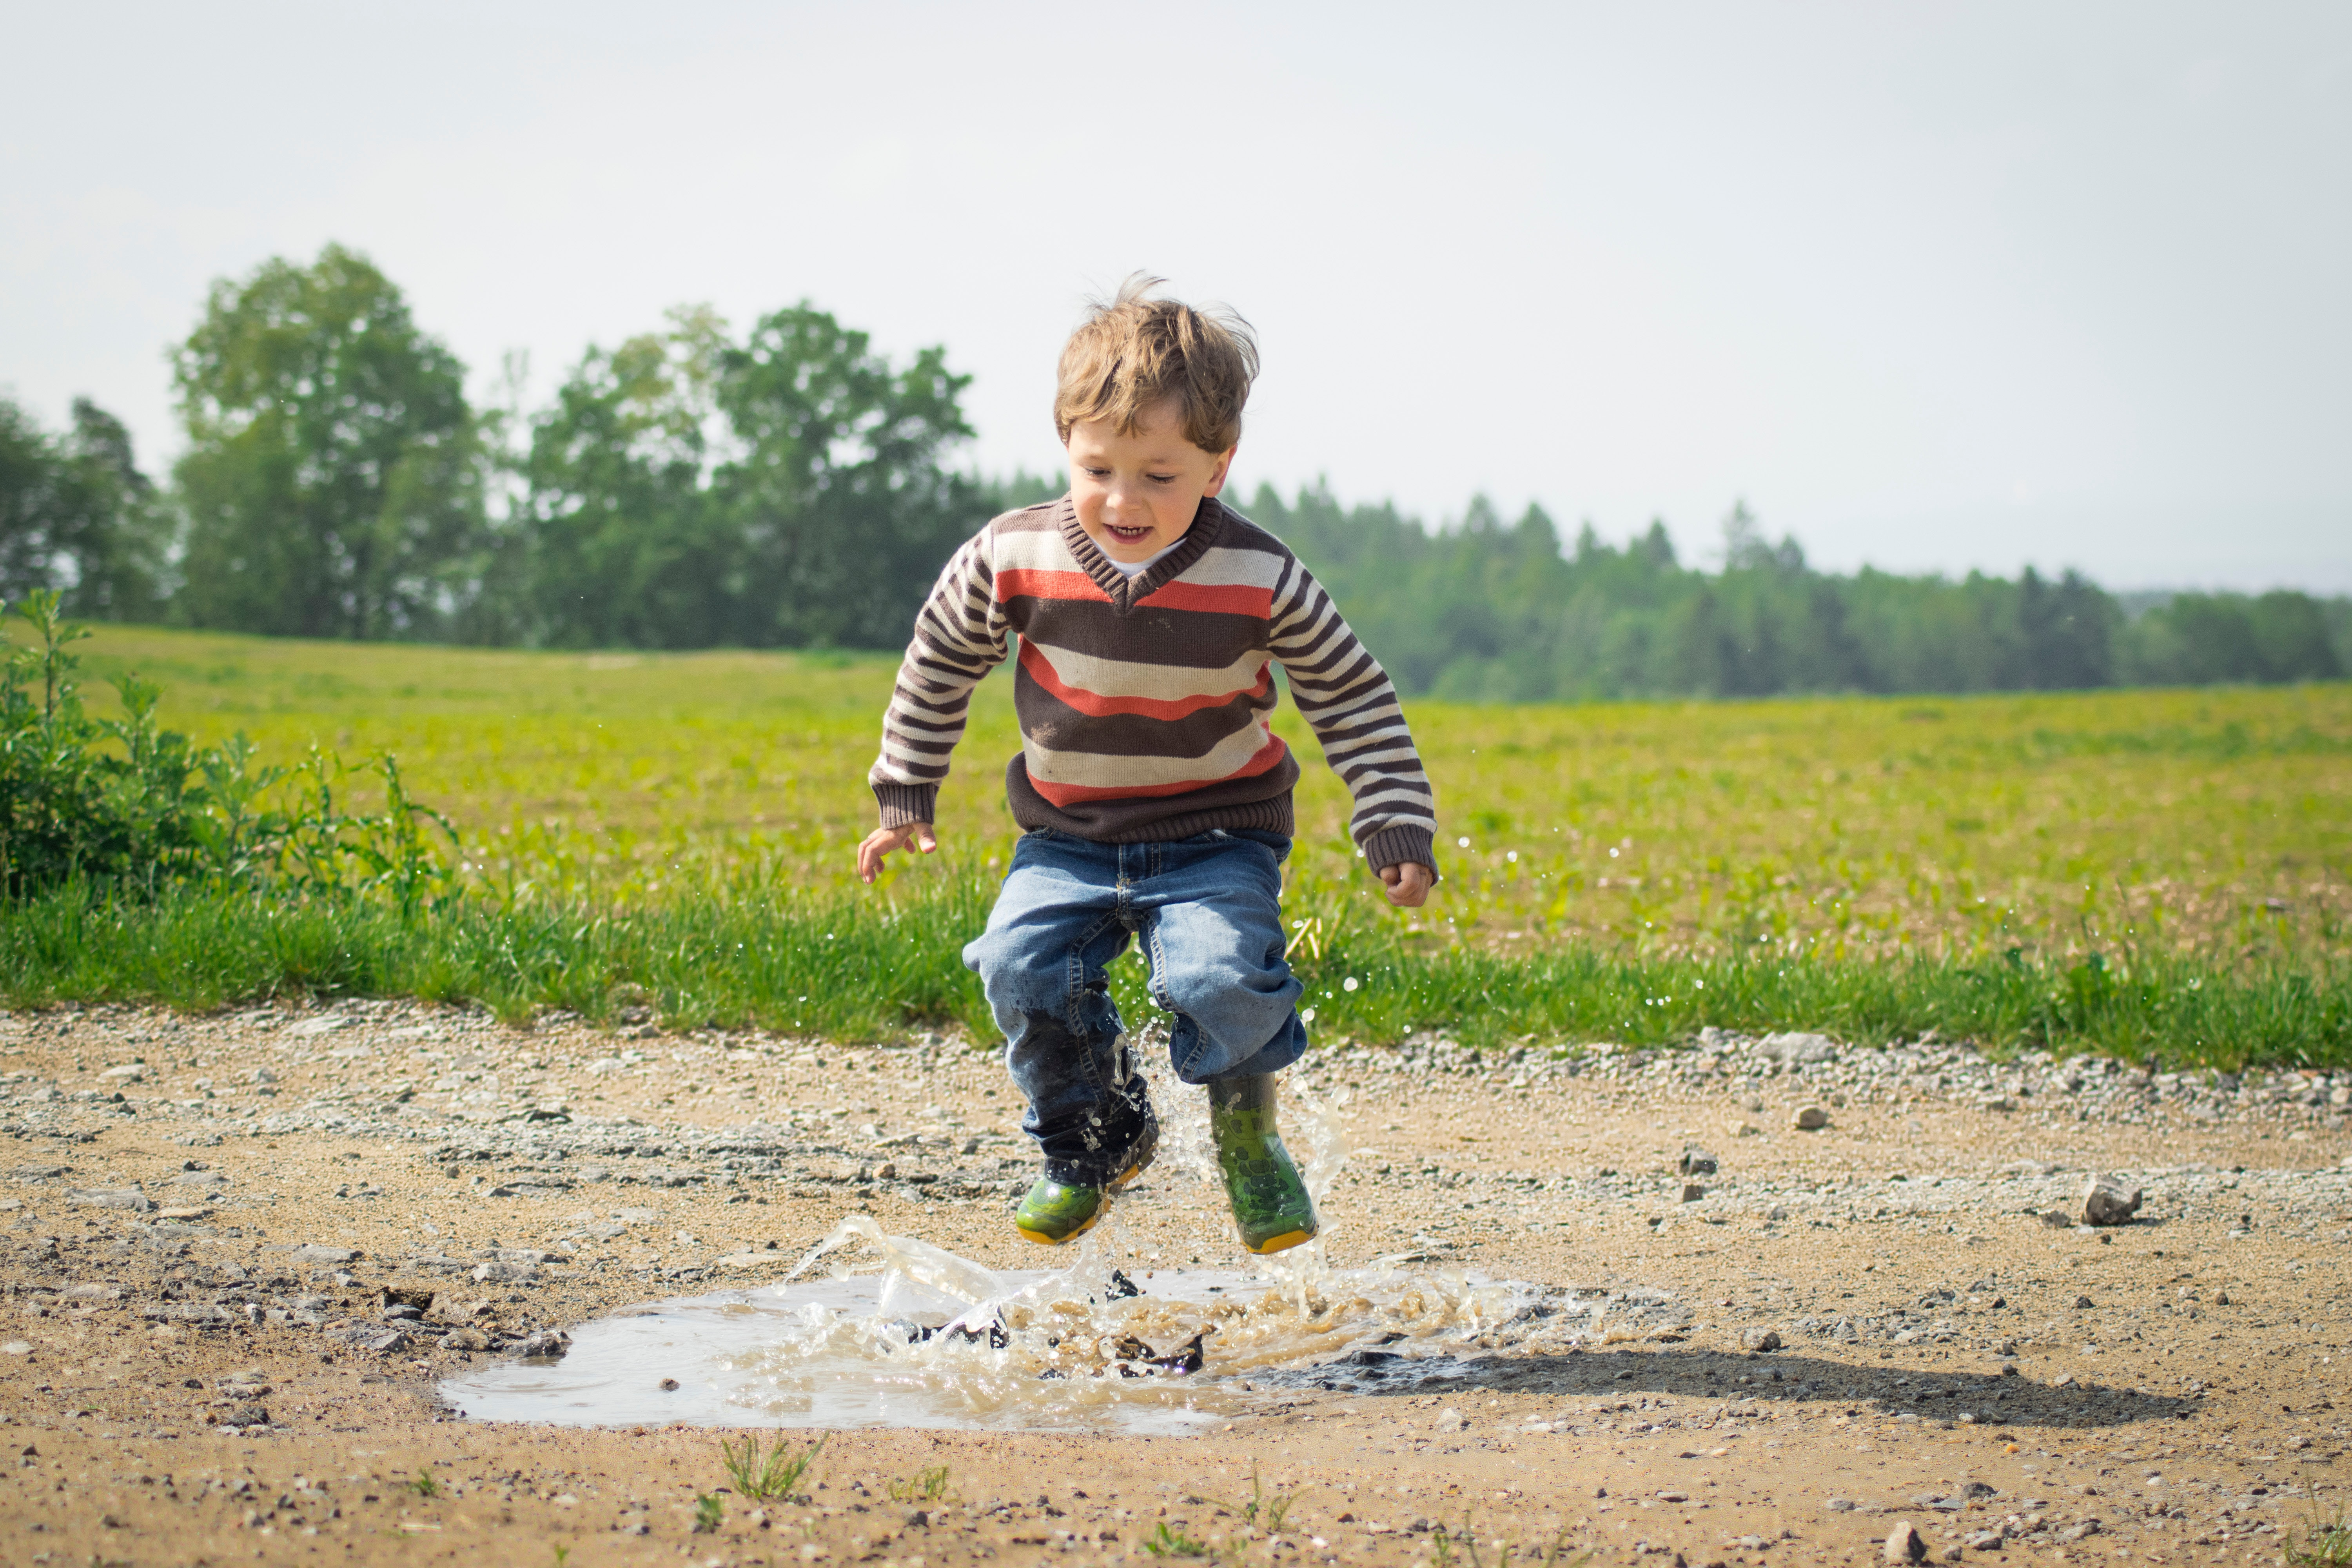
\includegraphics[width=.7\linewidth]{Fotosstest/3.jpg}
        \caption{Foto 5}
    \end{subfigure}%
    \begin{subfigure}{0.45\textwidth}
        \centering
        \includegraphics[width=.7\linewidth]{Fotosstest/4.jpg}
        \caption{Foto 6}
    \end{subfigure}
\end{figure}
\begin{figure}[h]
    \centering
    \begin{subfigure}{0.45\textwidth}
        \centering
        \includegraphics[width=.7\linewidth]{Fotosstest/5.jpg}
        \caption{Foto 7}
    \end{subfigure}%
    \begin{subfigure}{0.45\textwidth}
        \centering
        \includegraphics[width=.7\linewidth]{Fotosstest/6.jpg}
        \caption{Foto 8}
    \end{subfigure}
\end{figure}
\begin{figure}[h]
    \centering
    \begin{subfigure}{0.45\textwidth}
        \centering
        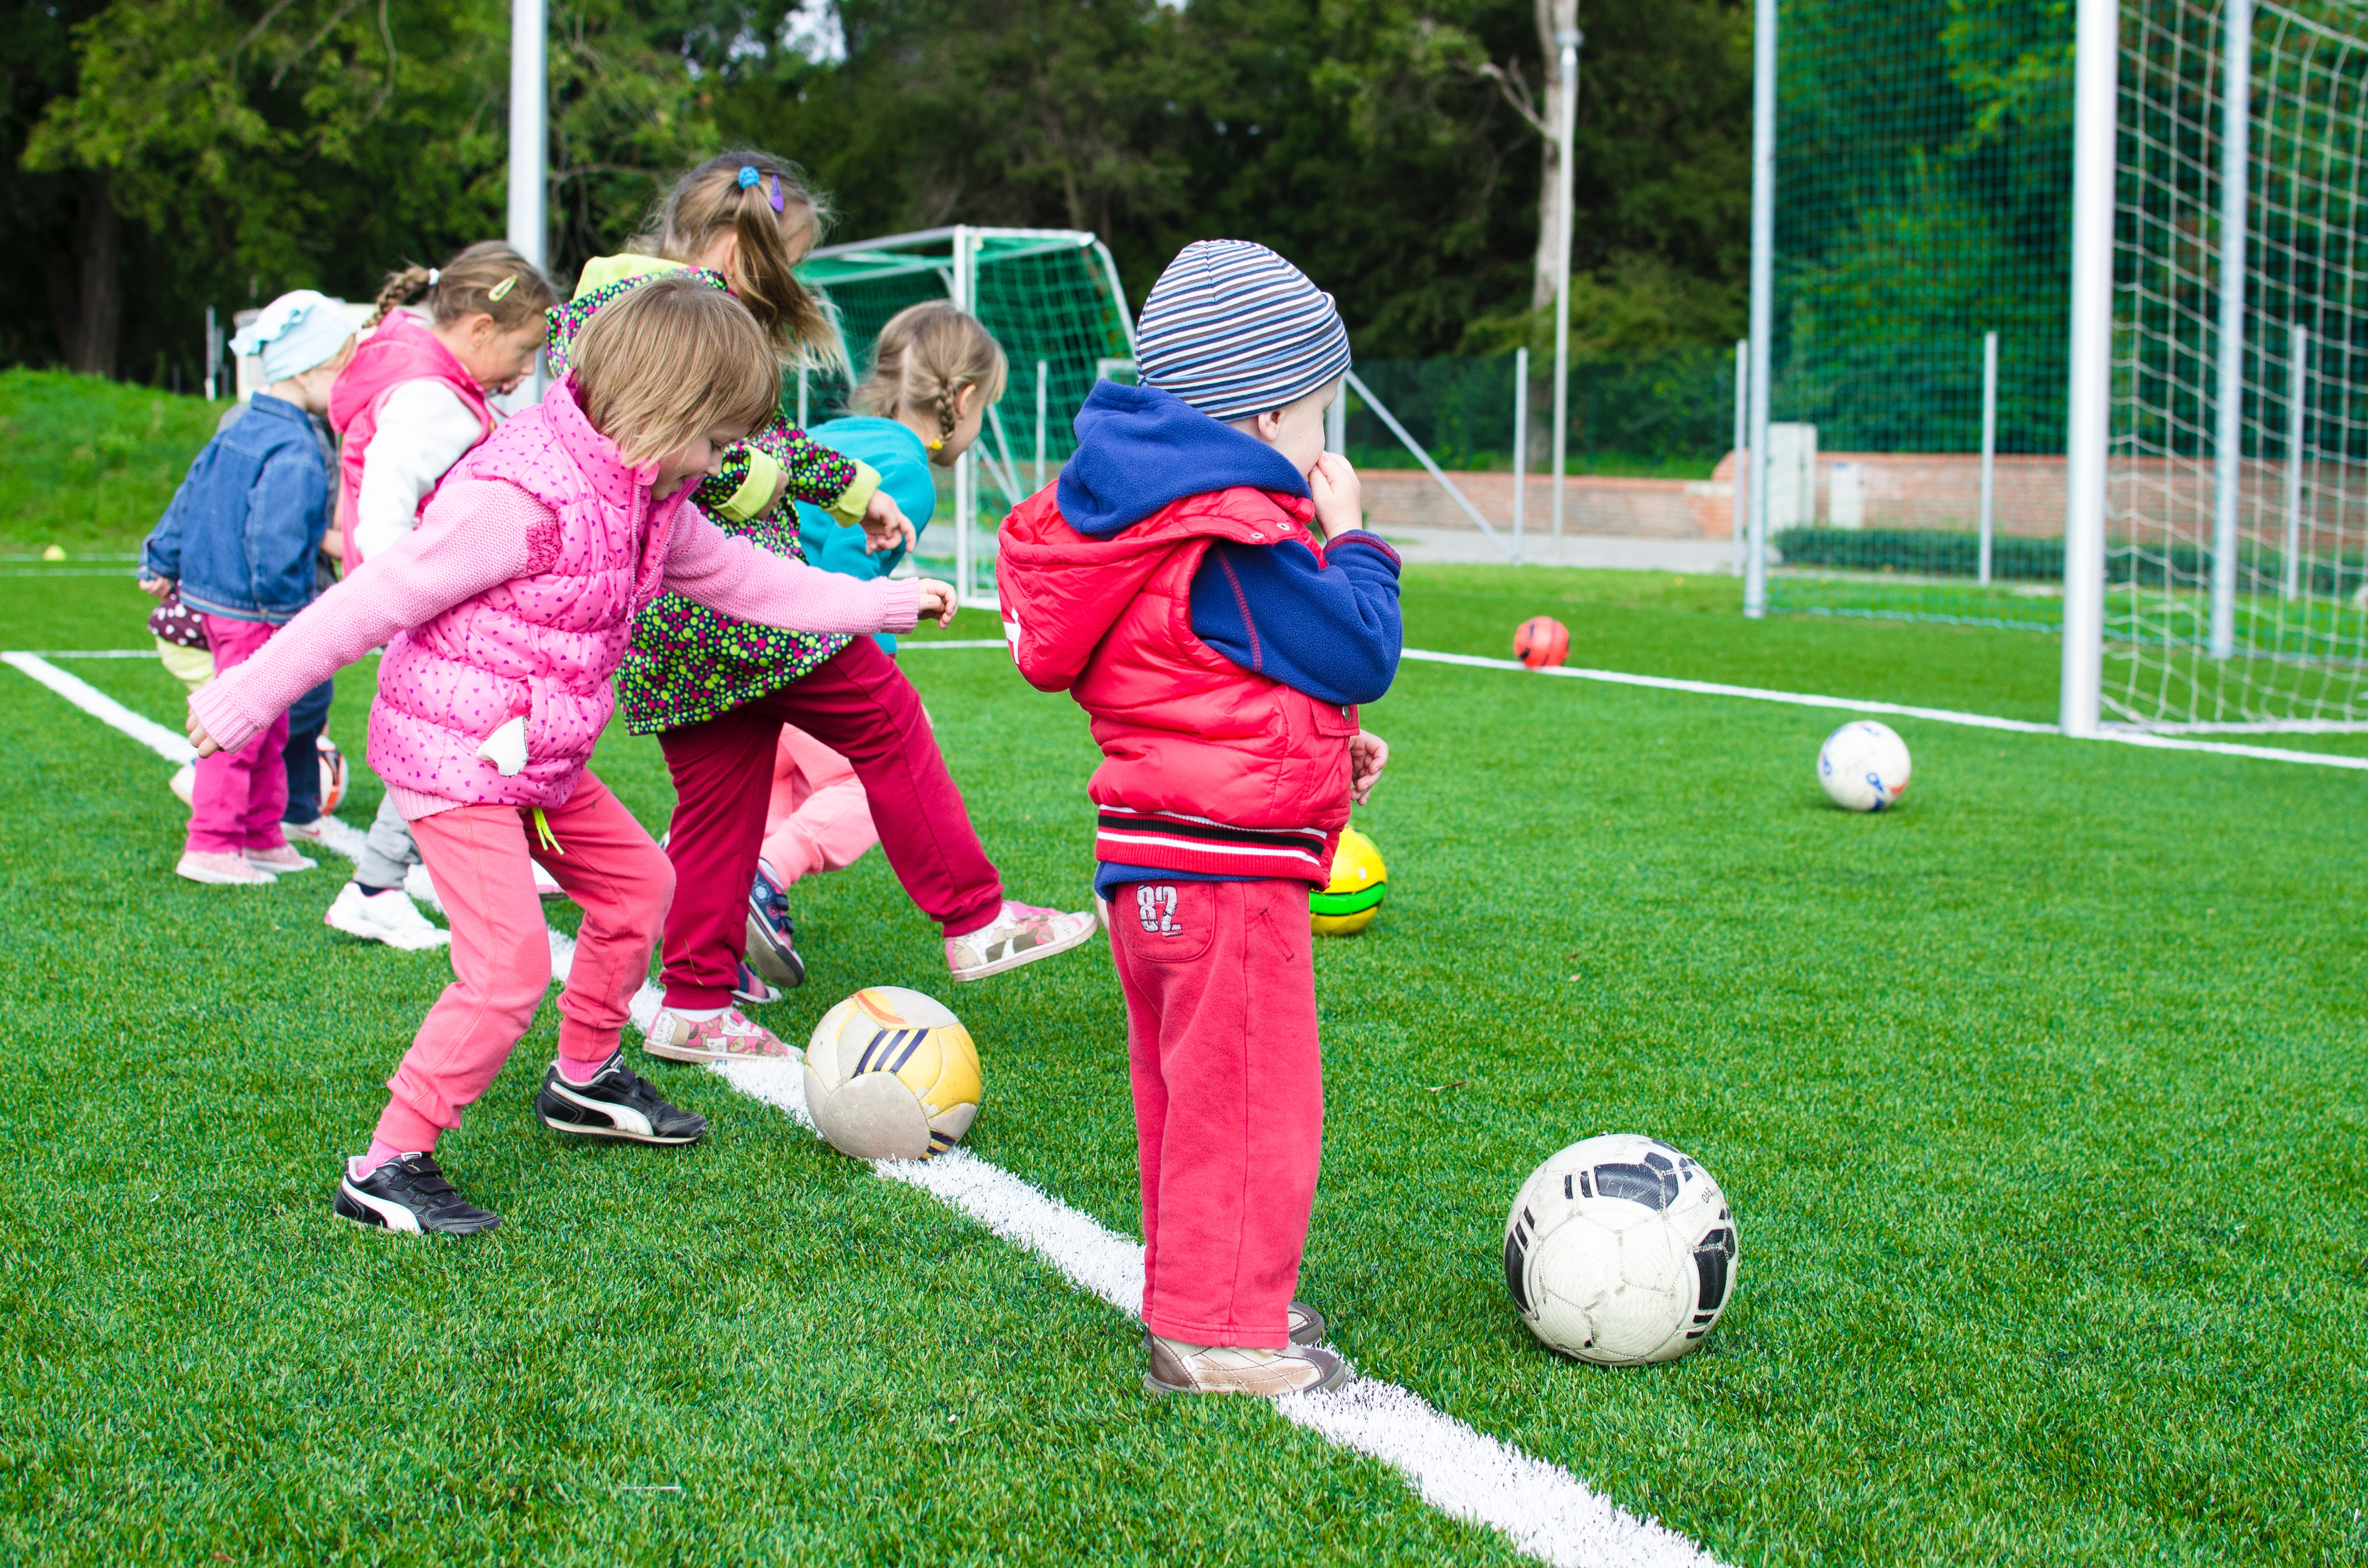
\includegraphics[width=.7\linewidth]{Fotosstest/7.jpg}
        \caption{Foto 9}
    \end{subfigure}%
    \begin{subfigure}{0.45\textwidth}
        \centering
        \includegraphics[width=.7\linewidth]{Fotosstest/8.jpg}
        \caption{Foto 10}
    \end{subfigure}
\end{figure}
\begin{figure}[h]
    \centering
    \begin{subfigure}{0.45\textwidth}
        \centering
        \includegraphics[width=.7\linewidth]{Fotosstest/9.jpg}
        \caption{Foto 11}
    \end{subfigure}%
    \begin{subfigure}{0.45\textwidth}
        \centering
        \includegraphics[width=.7\linewidth]{Fotosstest/10.jpg}
        \caption{Foto12}
    \end{subfigure}
\end{figure}
\begin{figure}[h]
    \centering
    \begin{subfigure}{0.45\textwidth}
        \centering
        \includegraphics[width=.7\linewidth]{Fotosstest/11.jpg}
        \caption{Foto 13}
    \end{subfigure}%
    \begin{subfigure}{0.45\textwidth}
        \centering
        \includegraphics[width=.7\linewidth]{Fotosstest/12.jpg}
        \caption{Foto 14}
    \end{subfigure}
\end{figure}
\begin{figure}[h]
    \centering
    \begin{subfigure}{0.45\textwidth}
        \centering
        \includegraphics[width=.7\linewidth]{Fotosstest/13.jpg}
        \caption{Foto 15}
    \end{subfigure}%
    \begin{subfigure}{0.45\textwidth}
        \centering
        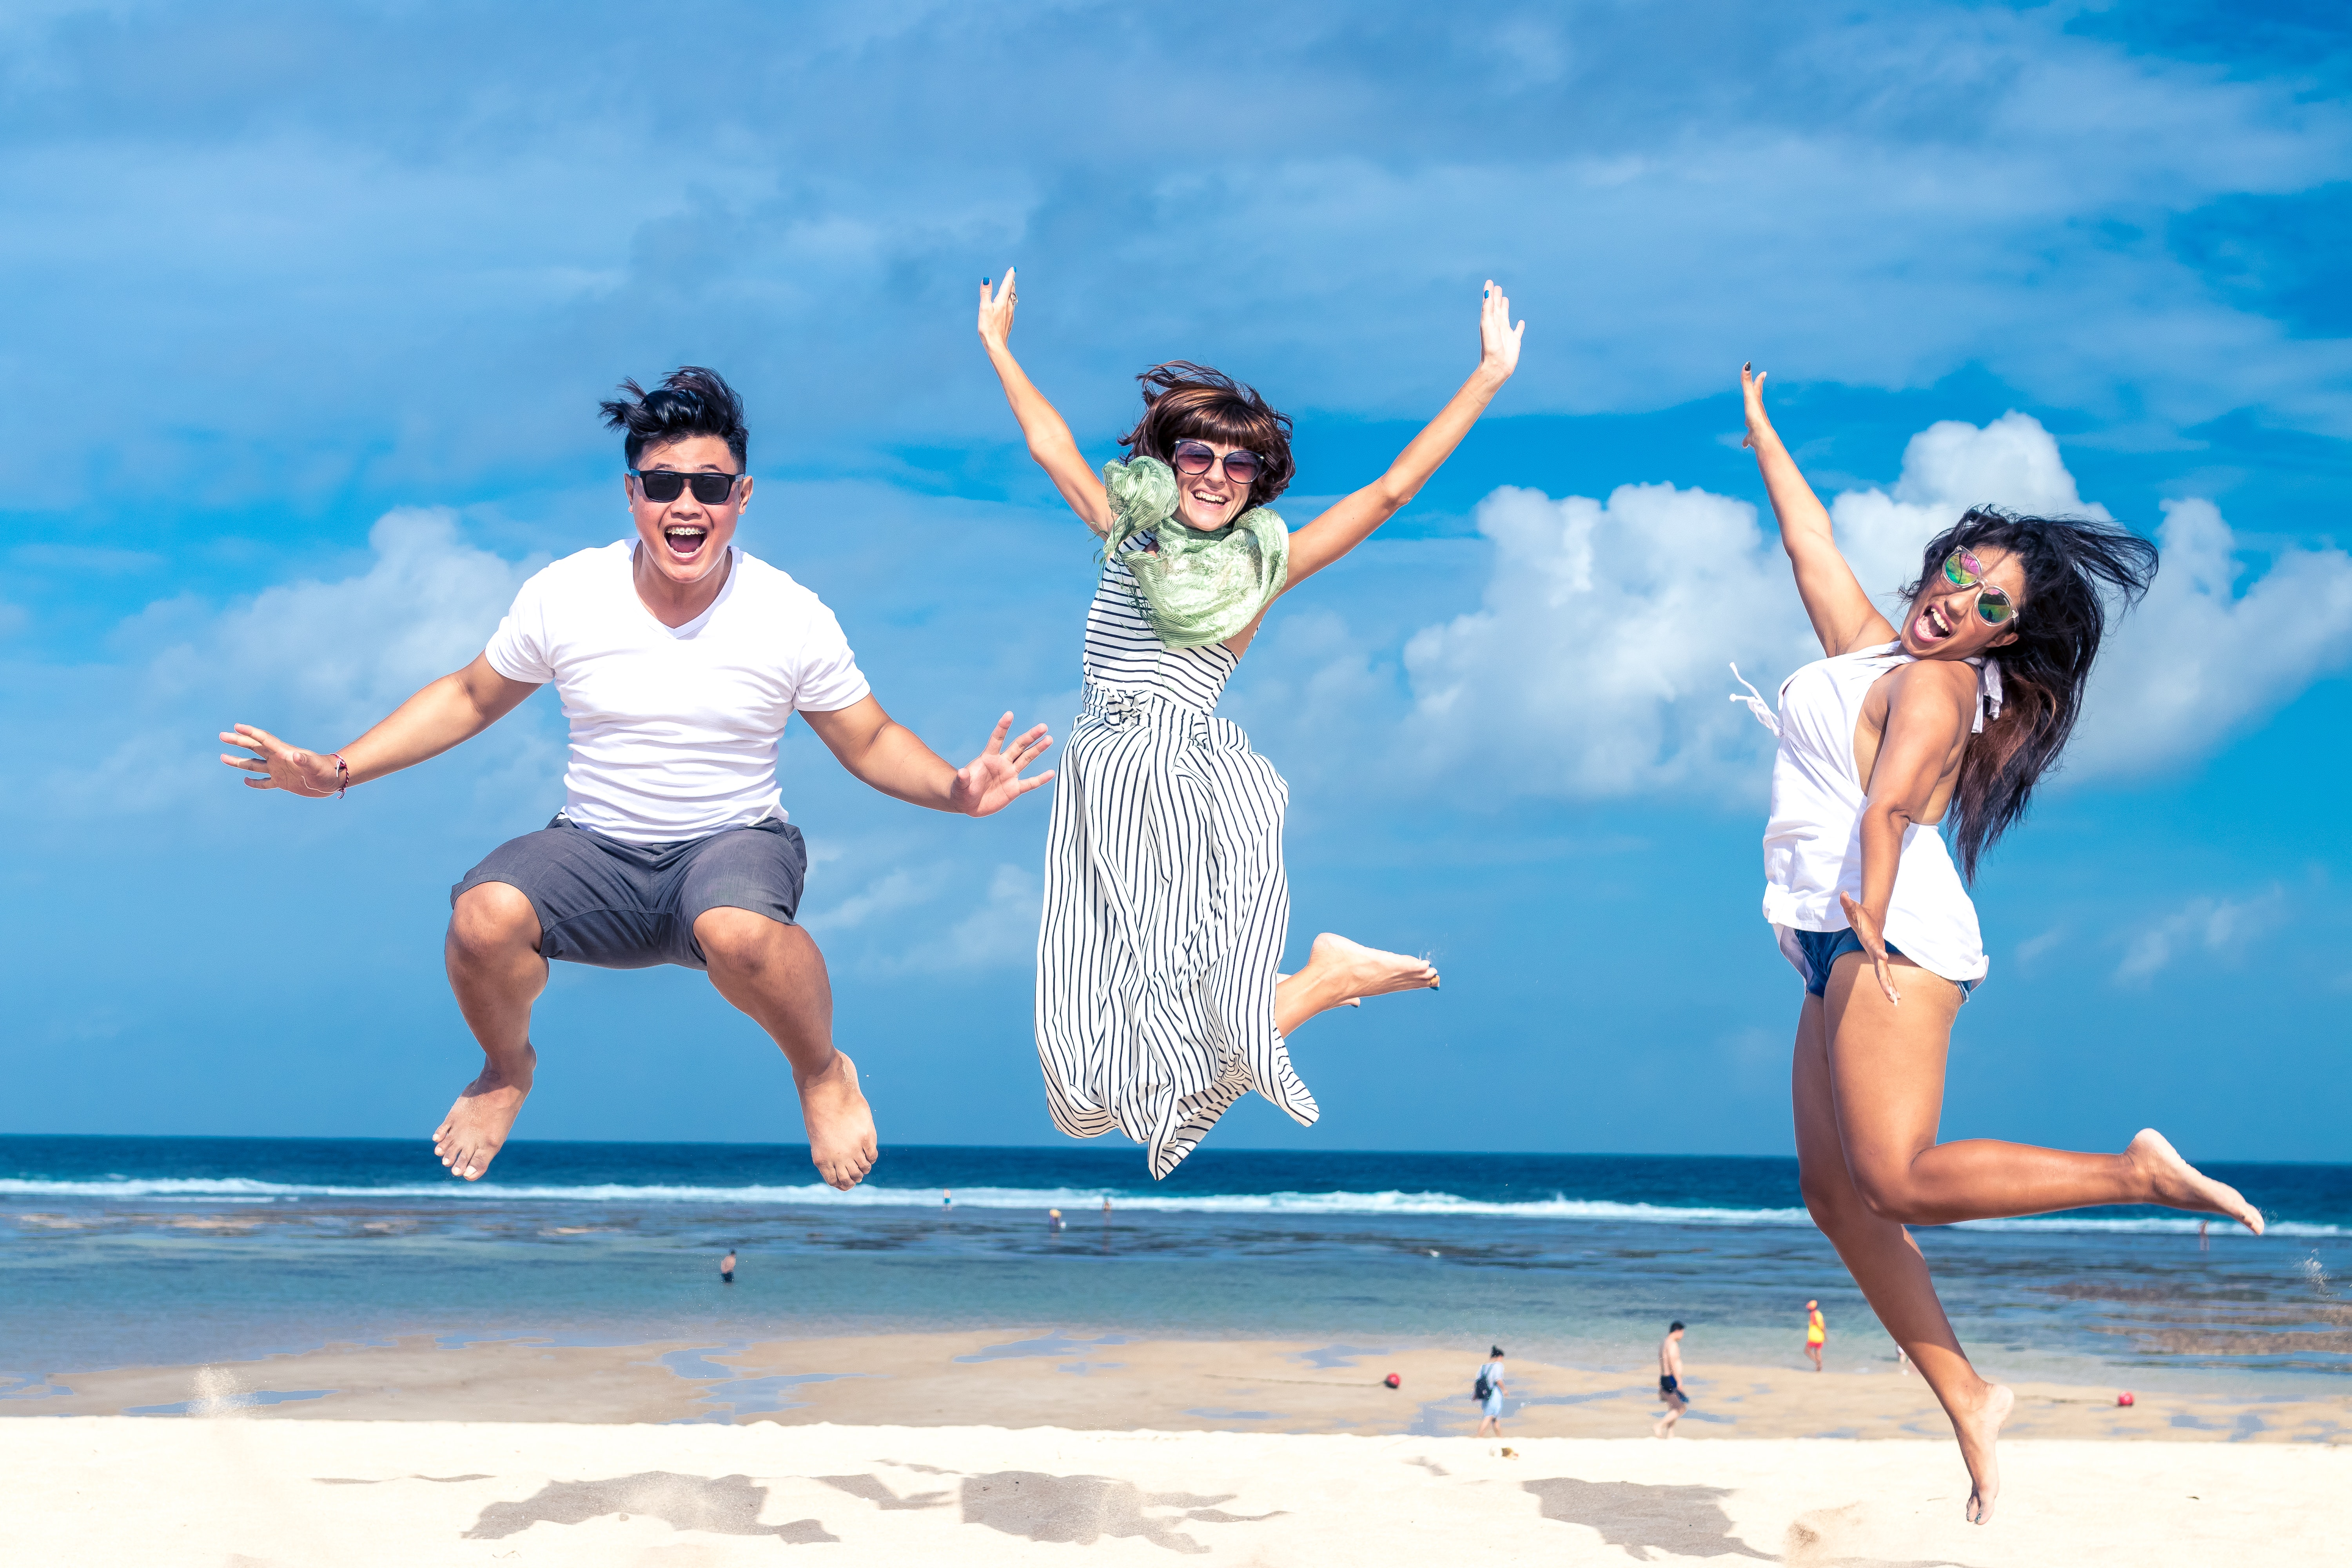
\includegraphics[width=.7\linewidth]{Fotosstest/14.jpg}
        \caption{Foto 16}
    \end{subfigure}
\end{figure}
\begin{figure}[h]
    \centering
    \begin{subfigure}{0.45\textwidth}
        \centering
        \includegraphics[width=.7\linewidth]{Fotosstest/15.jpg}
        \caption{Foto 17}
    \end{subfigure}%
    \begin{subfigure}{0.45\textwidth}
        \centering
        \includegraphics[width=.7\linewidth]{Fotosstest/16.jpg}
        \caption{Foto 18}
    \end{subfigure}
\end{figure}
\begin{figure}[h]
    \centering
    \begin{subfigure}{0.45\textwidth}
        \centering
        \includegraphics[width=.7\linewidth]{Fotosstest/17.jpg}
        \caption{Foto 19}
    \end{subfigure}%
    \begin{subfigure}{0.45\textwidth}
        \centering
        \includegraphics[width=.7\linewidth]{Fotosstest/18.jpg}
        \caption{Foto 20}
    \end{subfigure}
\end{figure}
\begin{figure}[h]
    \centering
    \begin{subfigure}{0.45\textwidth}
        \centering
        \includegraphics[width=.7\linewidth]{Fotosstest/19.jpg}
        \caption{Foto 21}
    \end{subfigure}%
    \begin{subfigure}{0.45\textwidth}
        \centering
        \includegraphics[width=.7\linewidth]{Fotosstest/20.jpg}
        \caption{Foto 22}
    \end{subfigure}
\end{figure}
\begin{figure}[h]
    \centering
    \begin{subfigure}{0.45\textwidth}
        \centering
        \includegraphics[width=.7\linewidth]{Fotosstest/21.jpg}
        \caption{Foto 23}
    \end{subfigure}%
    \begin{subfigure}{0.45\textwidth}
        \centering
        \includegraphics[width=.7\linewidth]{Fotosstest/22.jpg}
        \caption{Foto 24}
    \end{subfigure}
\end{figure}
\begin{figure}[h]
    \centering
    \begin{subfigure}{0.45\textwidth}
        \centering
        \includegraphics[width=.7\linewidth]{Fotosstest/23.jpg}
        \caption{Foto 25}
    \end{subfigure}%
    \begin{subfigure}{0.45\textwidth}
        \centering
        \includegraphics[width=.7\linewidth]{Fotosstest/24.jpg}
        \caption{Foto 26}
    \end{subfigure}
\end{figure}
\begin{figure}[h]
    \centering
    \begin{subfigure}{0.45\textwidth}
        \centering
        \includegraphics[width=.7\linewidth]{Fotosstest/25.jpg}
        \caption{Foto 27}
    \end{subfigure}%
    \begin{subfigure}{0.45\textwidth}
        \centering
        \includegraphics[width=.7\linewidth]{Fotosstest/26.jpg}
        \caption{Foto 28}
    \end{subfigure}
\end{figure}
\begin{figure}[h]
    \centering
    \begin{subfigure}{0.45\textwidth}
        \centering
        \includegraphics[width=.7\linewidth]{Fotosstest/27.jpg}
        \caption{Foto 29}
    \end{subfigure}%
    \begin{subfigure}{0.45\textwidth}
        \centering
        \includegraphics[width=.7\linewidth]{Fotosstest/28.jpg}
        \caption{Foto 30}
    \end{subfigure}
\end{figure}
\begin{figure}[h]
    \centering
    \begin{subfigure}{0.45\textwidth}
        \centering
        \includegraphics[width=.7\linewidth]{Fotosstest/29.jpg}
        \caption{Foto 31}
    \end{subfigure}%
    \begin{subfigure}{0.45\textwidth}
        \centering
        \includegraphics[width=.7\linewidth]{Fotosstest/30.jpg}
        \caption{Foto 32}
    \end{subfigure}
\end{figure}
\begin{figure}[h]
    \centering
    \begin{subfigure}{0.45\textwidth}
        \centering
        \includegraphics[width=.7\linewidth]{Fotosstest/31.jpg}
        \caption{Foto 33}
    \end{subfigure}%
    \begin{subfigure}{0.45\textwidth}
        \centering
        \includegraphics[width=.7\linewidth]{Fotosstest/32.jpg}
        \caption{Foto 34}
    \end{subfigure}
\end{figure}
\begin{figure}[h]
    \centering
    \begin{subfigure}{0.45\textwidth}
        \centering
        \includegraphics[width=.7\linewidth]{Fotosstest/33.jpg}
        \caption{Foto 35}
    \end{subfigure}%
    \begin{subfigure}{0.45\textwidth}
        \centering
        \includegraphics[width=.7\linewidth]{Fotosstest/34.jpg}
        \caption{Foto 36}
    \end{subfigure}
\end{figure}
\begin{figure}[h]
    \centering
    \begin{subfigure}{0.45\textwidth}
        \centering
        \includegraphics[width=.7\linewidth]{Fotosstest/35.jpg}
        \caption{Foto 37}
    \end{subfigure}%
    \begin{subfigure}{0.45\textwidth}
        \centering
        \includegraphics[width=.7\linewidth]{Fotosstest/36.jpg}
        \caption{Foto 38}
    \end{subfigure}
\end{figure}
\begin{figure}[h]
    \centering
    \begin{subfigure}{0.45\textwidth}
        \centering
        \includegraphics[width=.7\linewidth]{Fotosstest/37.jpg}
        \caption{Foto 39}
    \end{subfigure}%
    \begin{subfigure}{0.45\textwidth}
        \centering
        \includegraphics[width=.7\linewidth]{Fotosstest/38.jpg}
        \caption{Foto 40}
    \end{subfigure}
\end{figure}

%%---------- Referentielijst --------------------------------------------------

\printbibliography[heading=bibintoc]

\end{document}
